\documentclass[12pt,a4paper]{article}
\usepackage{ctex}
\title{基于Transformer的神经机器翻译实验报告}
\author{}

\usepackage{hyperref}
\hypersetup{colorlinks=true, linkcolor=blue, anchorcolor=green, citecolor=green}
\usepackage{bm}
\usepackage{amssymb, amsmath, amsthm}
\usepackage{graphicx}
\usepackage{float}
\usepackage{booktabs}
\usepackage{longtable}
\usepackage{multirow}
\usepackage{subcaption}
\usepackage{listings}
\usepackage{xcolor}
\usepackage{enumitem}

\lstset{
    language=Python,
    basicstyle=\ttfamily\small,
    keywordstyle=\color{blue},
    commentstyle=\color{gray},
    stringstyle=\color{red},
    breaklines=true,
    frame=single,
    numbers=left,
    numberstyle=\tiny\color{gray}
}

\begin{document}

\begin{titlepage}
    \centering
    \vspace*{1cm}
    
\includegraphics[width=0.6\textwidth]{ucas_logo.pdf}
    \vspace{1cm}

    {\Huge\bfseries 深度学习作业4\par}
    \vspace{1cm}
    {\LARGE 基于Transformer的神经机器翻译实验\par}
    \vspace{3cm}

    \begin{tabular}{rl}
        {\kaishu\Large 学号：} & {\kaishu\Large \underline{\makebox[6cm]{202528014629014}}} \\[0.8cm]
        {\kaishu\Large 姓名：} & {\kaishu\Large \underline{\makebox[6cm]{刘浩}}} \\[0.8cm]
        {\kaishu\Large 院所：} & {\kaishu\Large \underline{\makebox[6cm]{人工智能学院}}} \\[0.8cm]
    \end{tabular}

    \vfill
    {\large \today}
\end{titlepage}

\tableofcontents
\newpage

\section{实验目的}

本实验旨在通过实践掌握基于Transformer架构的序列到序列模型在机器翻译任务中的应用。Transformer完全依赖自注意力机制来捕捉序列中任意位置之间的依赖关系，相比循环神经网络在翻译质量和训练效率上都有显著提升。本实验在NiuTrans平行语料库上构建中英翻译系统，深入理解多头注意力、位置编码、标签平滑等关键技术的实际效果，目标是达到BLEU-4大于14的翻译质量。

\section{实验原理}

\subsection{Transformer架构}

Transformer模型由编码器和解码器两部分组成，每一部分均由多个相同的层堆叠而成。编码器的每一层包含多头自注意力子层和前馈网络子层，两者均通过残差连接和层归一化进行稳定训练。解码器在此基础上增加了编码器-解码器交叉注意力子层，使得解码过程能够关注到源语言的信息。

\subsection{自注意力机制}

自注意力的核心计算如下：
\begin{equation}
    \text{Attention}(Q, K, V) = \text{softmax}\left(\frac{QK^\top}{\sqrt{d_k}}\right)V
\end{equation}
其中$Q$、$K$、$V$分别是查询、键、值矩阵，$d_k$是键的维度。缩放因子$\sqrt{d_k}$防止点积过大导致softmax梯度消失。多头注意力则将输入投影到多个子空间分别计算注意力，再拼接结果：
\begin{equation}
    \text{MultiHead}(Q, K, V) = \text{Concat}(\text{head}_1, \ldots, \text{head}_h)W^O
\end{equation}

\subsection{位置编码}

由于Transformer不含循环结构，需要显式注入位置信息。本实验采用正弦余弦位置编码：
\begin{equation}
    PE_{(pos, 2i)} = \sin\left(\frac{pos}{10000^{2i/d_{model}}}\right), \quad
    PE_{(pos, 2i+1)} = \cos\left(\frac{pos}{10000^{2i/d_{model}}}\right)
\end{equation}
这种编码方式的优势在于模型可以通过线性变换关注到相对位置信息，且能够外推到训练中未见过的序列长度。

\subsection{标签平滑}

在训练过程中，我们使用标签平滑正则化技术，将目标分布从one-hot形式软化为：
\begin{equation}
    y_i^{ls} = (1 - \epsilon) \cdot y_i + \frac{\epsilon}{|V|}
\end{equation}
其中$\epsilon=0.1$。虽然会略微增加困惑度，但能有效防止模型对预测过于自信，从而提升泛化性能和BLEU分数。

\subsection{Noam学习率调度}

学习率采用warmup-then-decay的策略：
\begin{equation}
    lr = d_{model}^{-0.5} \cdot \min(step^{-0.5},\ step \cdot warmup\_steps^{-1.5})
\end{equation}
在warmup阶段学习率线性增长，之后按步数的平方根衰减。这种策略能够在训练初期稳定梯度更新，后期逐渐精细化参数。

\subsection{BLEU评估指标}

BLEU-4通过计算假设翻译与参考翻译之间1-gram到4-gram的精确率几何平均，并乘以简短惩罚因子来评估翻译质量：
\begin{equation}
    \text{BLEU} = BP \cdot \exp\left(\sum_{n=1}^{4} \frac{1}{4}\log p_n\right)
\end{equation}

\section{数据集分析}

本实验使用NiuTrans开源中英平行语料库，包含100,000个中英句子对作为训练集，400个句子对作为验证集，1000个中文句子（每个配有3个英文参考翻译）作为测试集。

\begin{figure}[H]
    \centering
    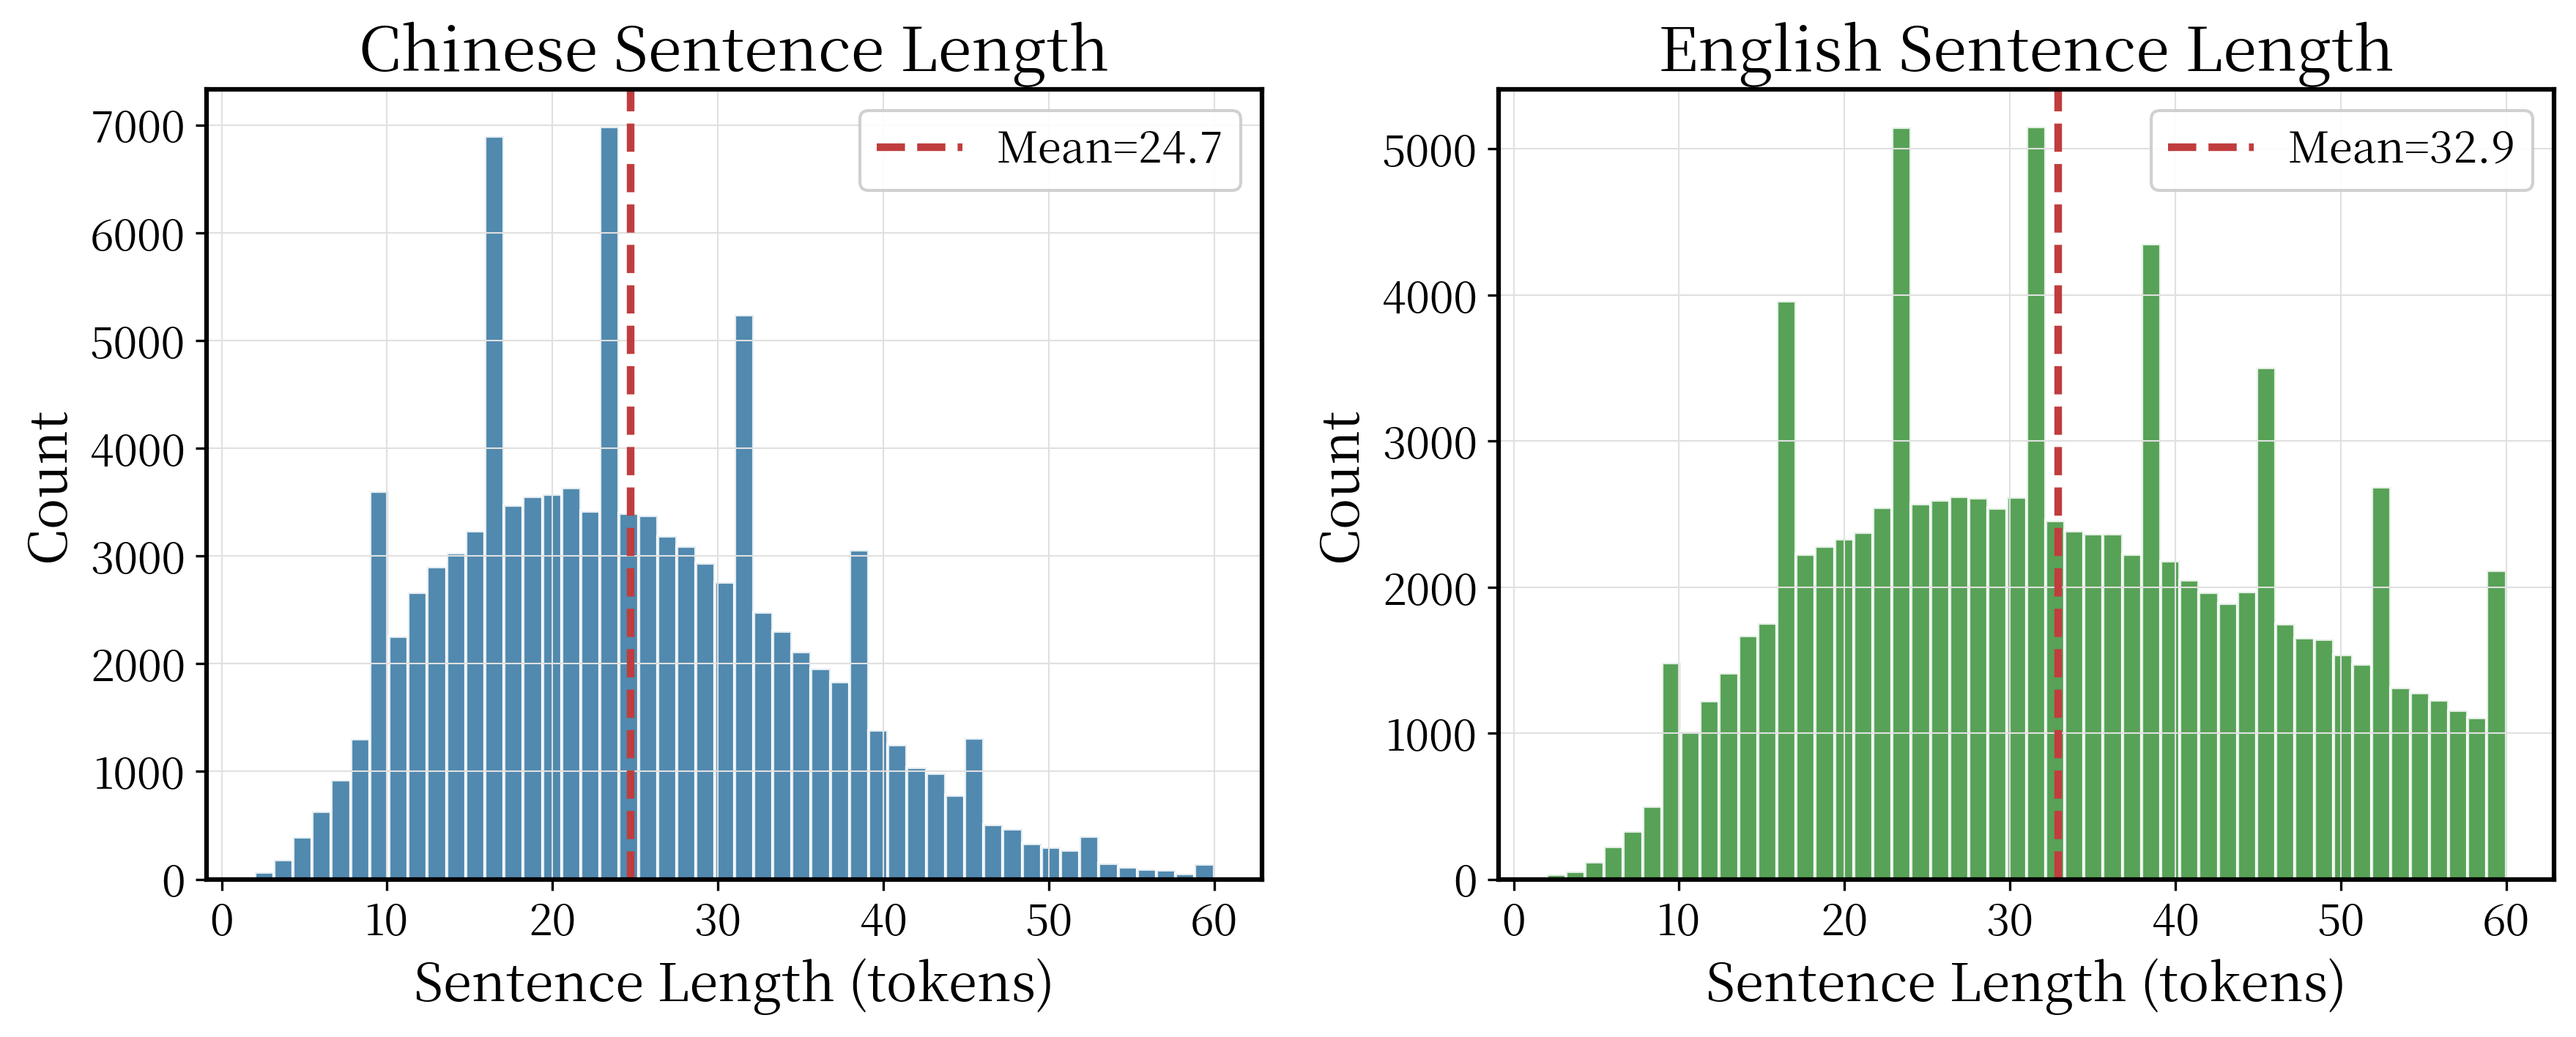
\includegraphics[width=0.95\textwidth]{figs/fig01_sentence_length.png}
    \caption{中英文句子长度分布。中文句子平均长度约为20个词，英文句子则更长，这反映了中英文在表达同一语义时的词汇密度差异。}
    \label{fig:sent_len}
\end{figure}

从图\ref{fig:sent_len}可以看出，中文句子的长度分布相对集中，而英文句子则呈现更长的尾部。这一特征意味着解码器在生成英文翻译时通常需要输出比源句更多的词元，这对模型的生成能力提出了更高要求。

\begin{figure}[H]
    \centering
    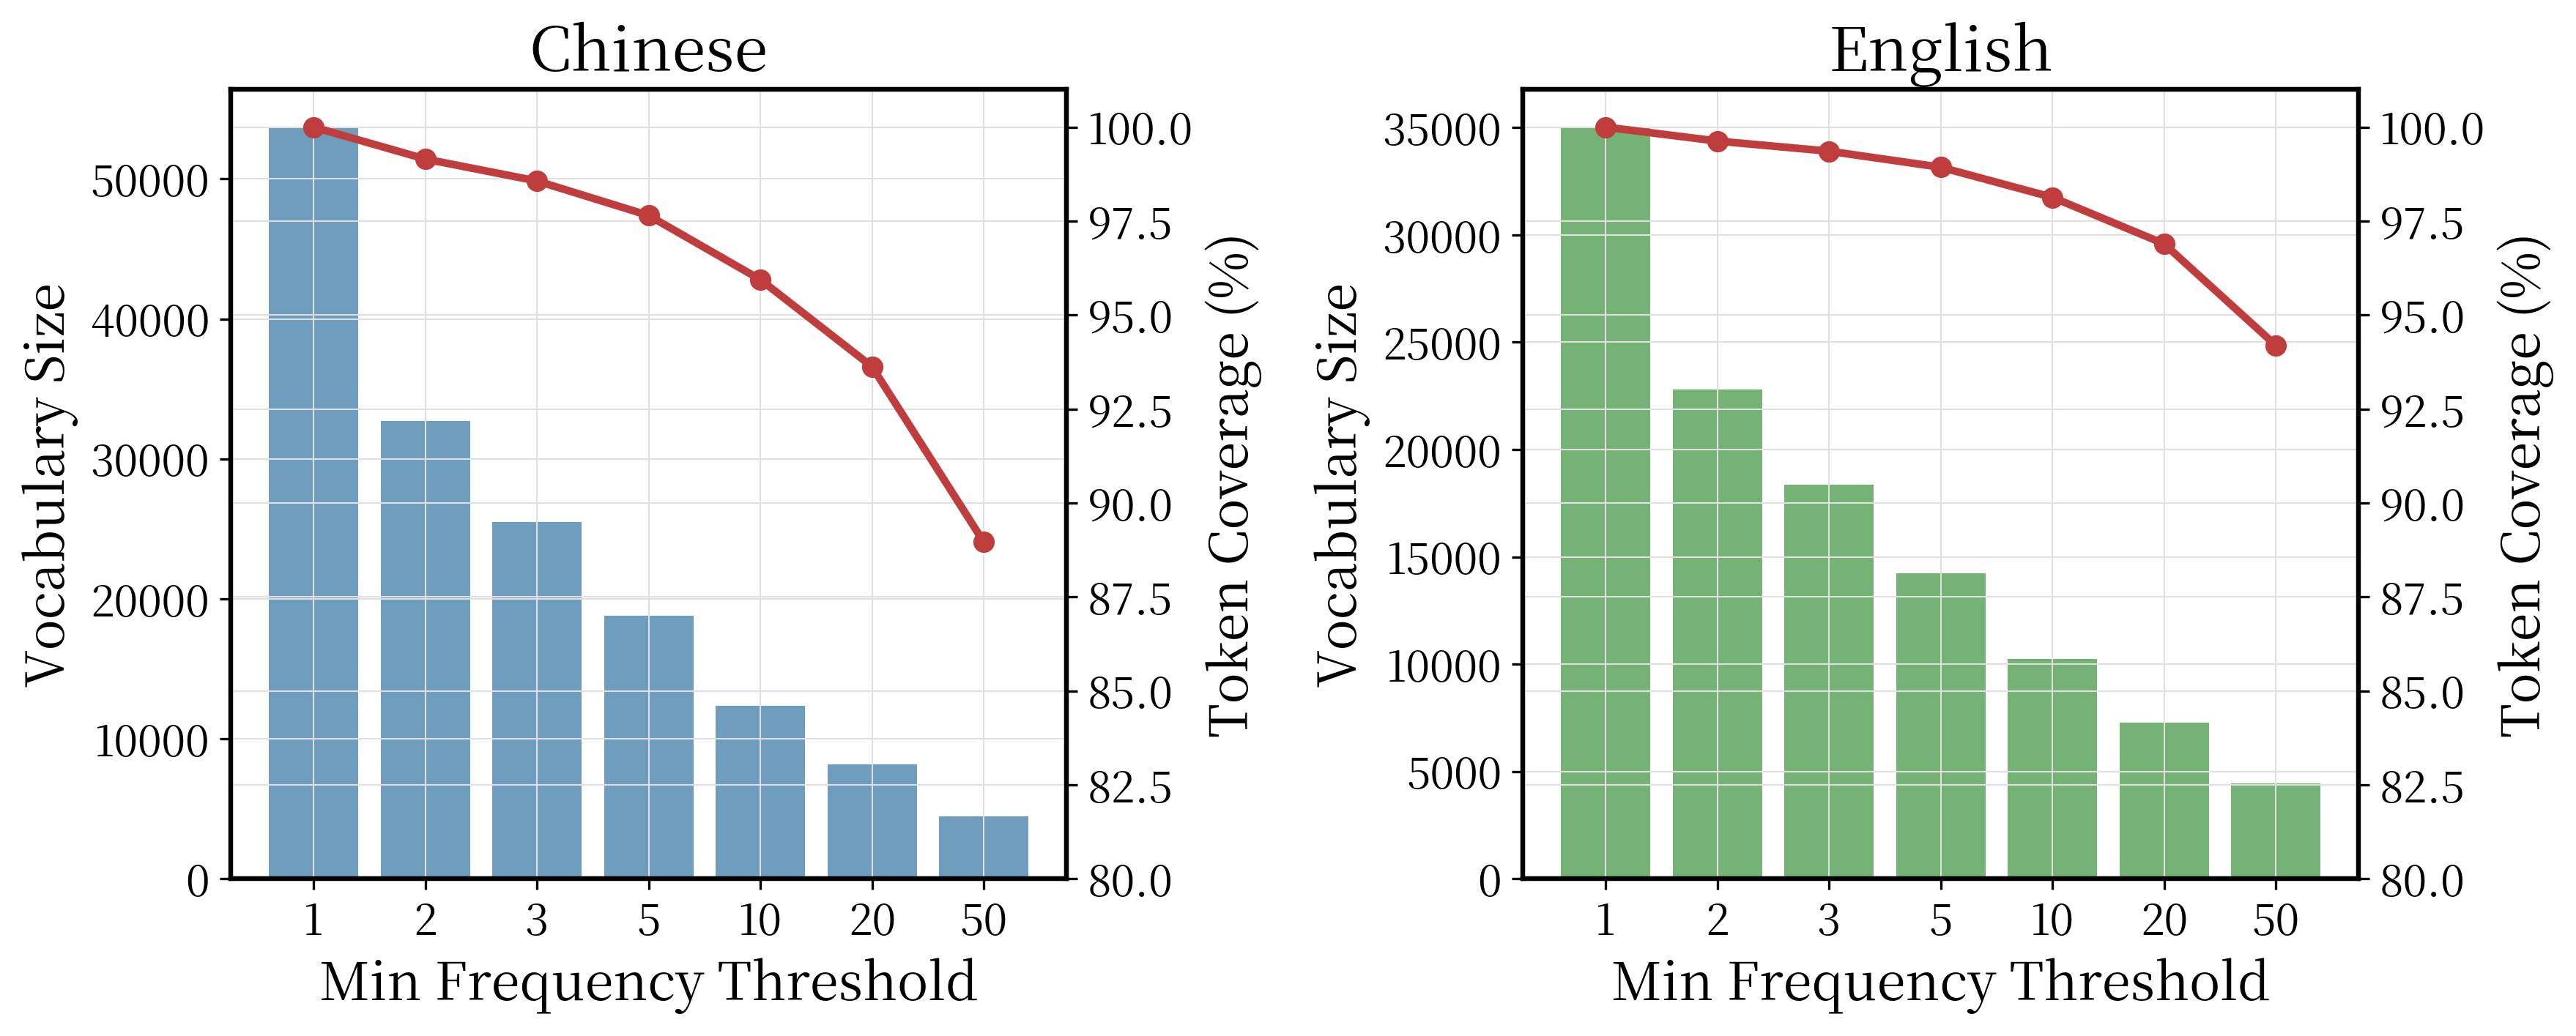
\includegraphics[width=0.95\textwidth]{figs/fig02_vocab_coverage.png}
    \caption{词频阈值与词表大小及覆盖率的关系}
    \label{fig:vocab}
\end{figure}

图\ref{fig:vocab}展示了在不同最低词频阈值下的词表大小和token覆盖率。我们选择最低词频为2作为过滤条件，在控制词表规模（约30,000）的同时保持了超过99\%的token覆盖率。

\begin{figure}[H]
    \centering
    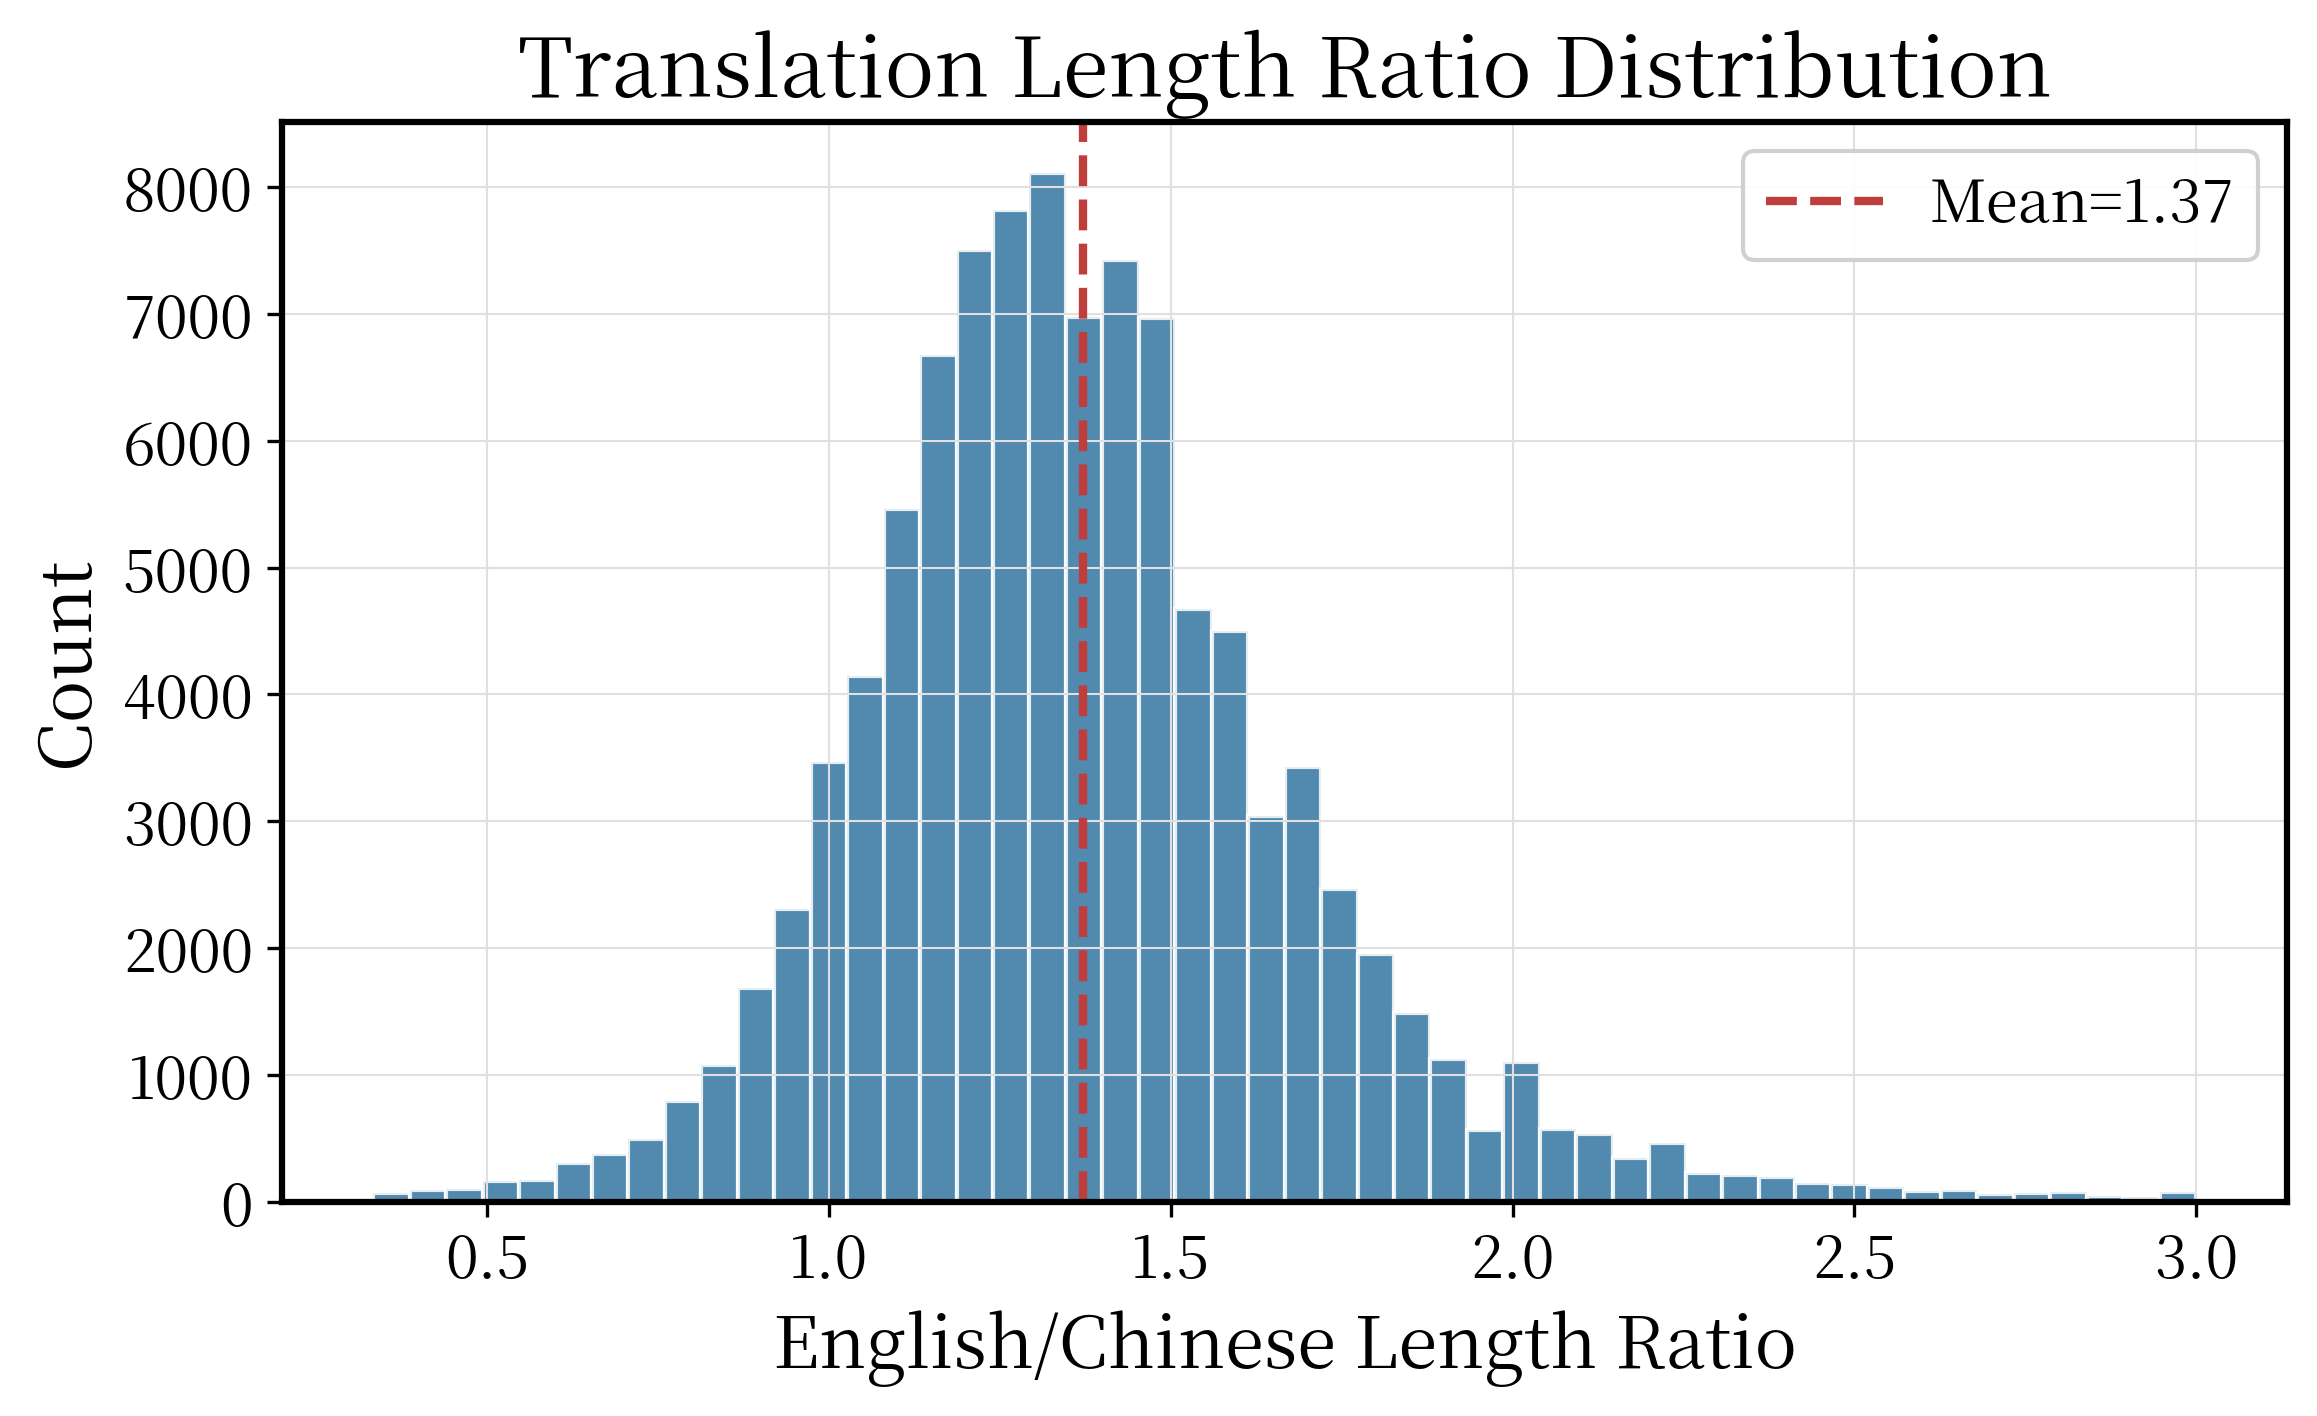
\includegraphics[width=0.7\textwidth]{figs/fig10_length_ratio.png}
    \caption{英中翻译长度比分布}
    \label{fig:ratio}
\end{figure}

图\ref{fig:ratio}展示了英中翻译长度比的分布。大部分句子对的英中长度比集中在1.0--1.5之间，说明英文翻译通常比中文源句更长，这与英文中介词、冠词等功能词较多的语言特性一致。模型在解码时需要学会适当地"扩展"输出长度，而非逐字对应翻译。

\section{模型设计与实现}

\subsection{模型配置}

为了探究模型规模对翻译质量的影响，本实验设计了三种不同规模的Transformer模型：

\begin{table}[H]
    \centering
    \begin{tabular}{lccccc}
        \toprule
        模型 & 层数 & $d_{model}$ & 注意力头数 & $d_{ff}$ & Dropout \\
        \midrule
        Small & 3 & 256 & 8 & 1024 & 0.1 \\
        Base & 6 & 512 & 8 & 2048 & 0.1 \\
        Large & 8 & 512 & 8 & 2048 & 0.15 \\
        \bottomrule
    \end{tabular}
    \caption{三种模型配置对比}
\end{table}

\subsection{训练策略}

所有模型均采用Adam优化器（$\beta_1=0.9$，$\beta_2=0.98$），配合Noam学习率调度。解码端以真实目标序列作为输入进行自回归训练，损失函数为标签平滑交叉熵，梯度裁剪范数设为1.0。最大序列长度限制为60个token，超长句子在数据预处理阶段被过滤。

\subsection{解码策略}

推理阶段我们对比了贪心解码和不同宽度的束搜索。束搜索在每一步保留$k$个最优候选序列，通过扩展每个候选并保留全局最优的$k$个路径来平衡搜索广度和效率。最终对候选序列按长度归一化的对数概率进行排序，选取最优翻译。

\section{实验结果与分析}

\subsection{训练过程}

\begin{figure}[H]
    \centering
    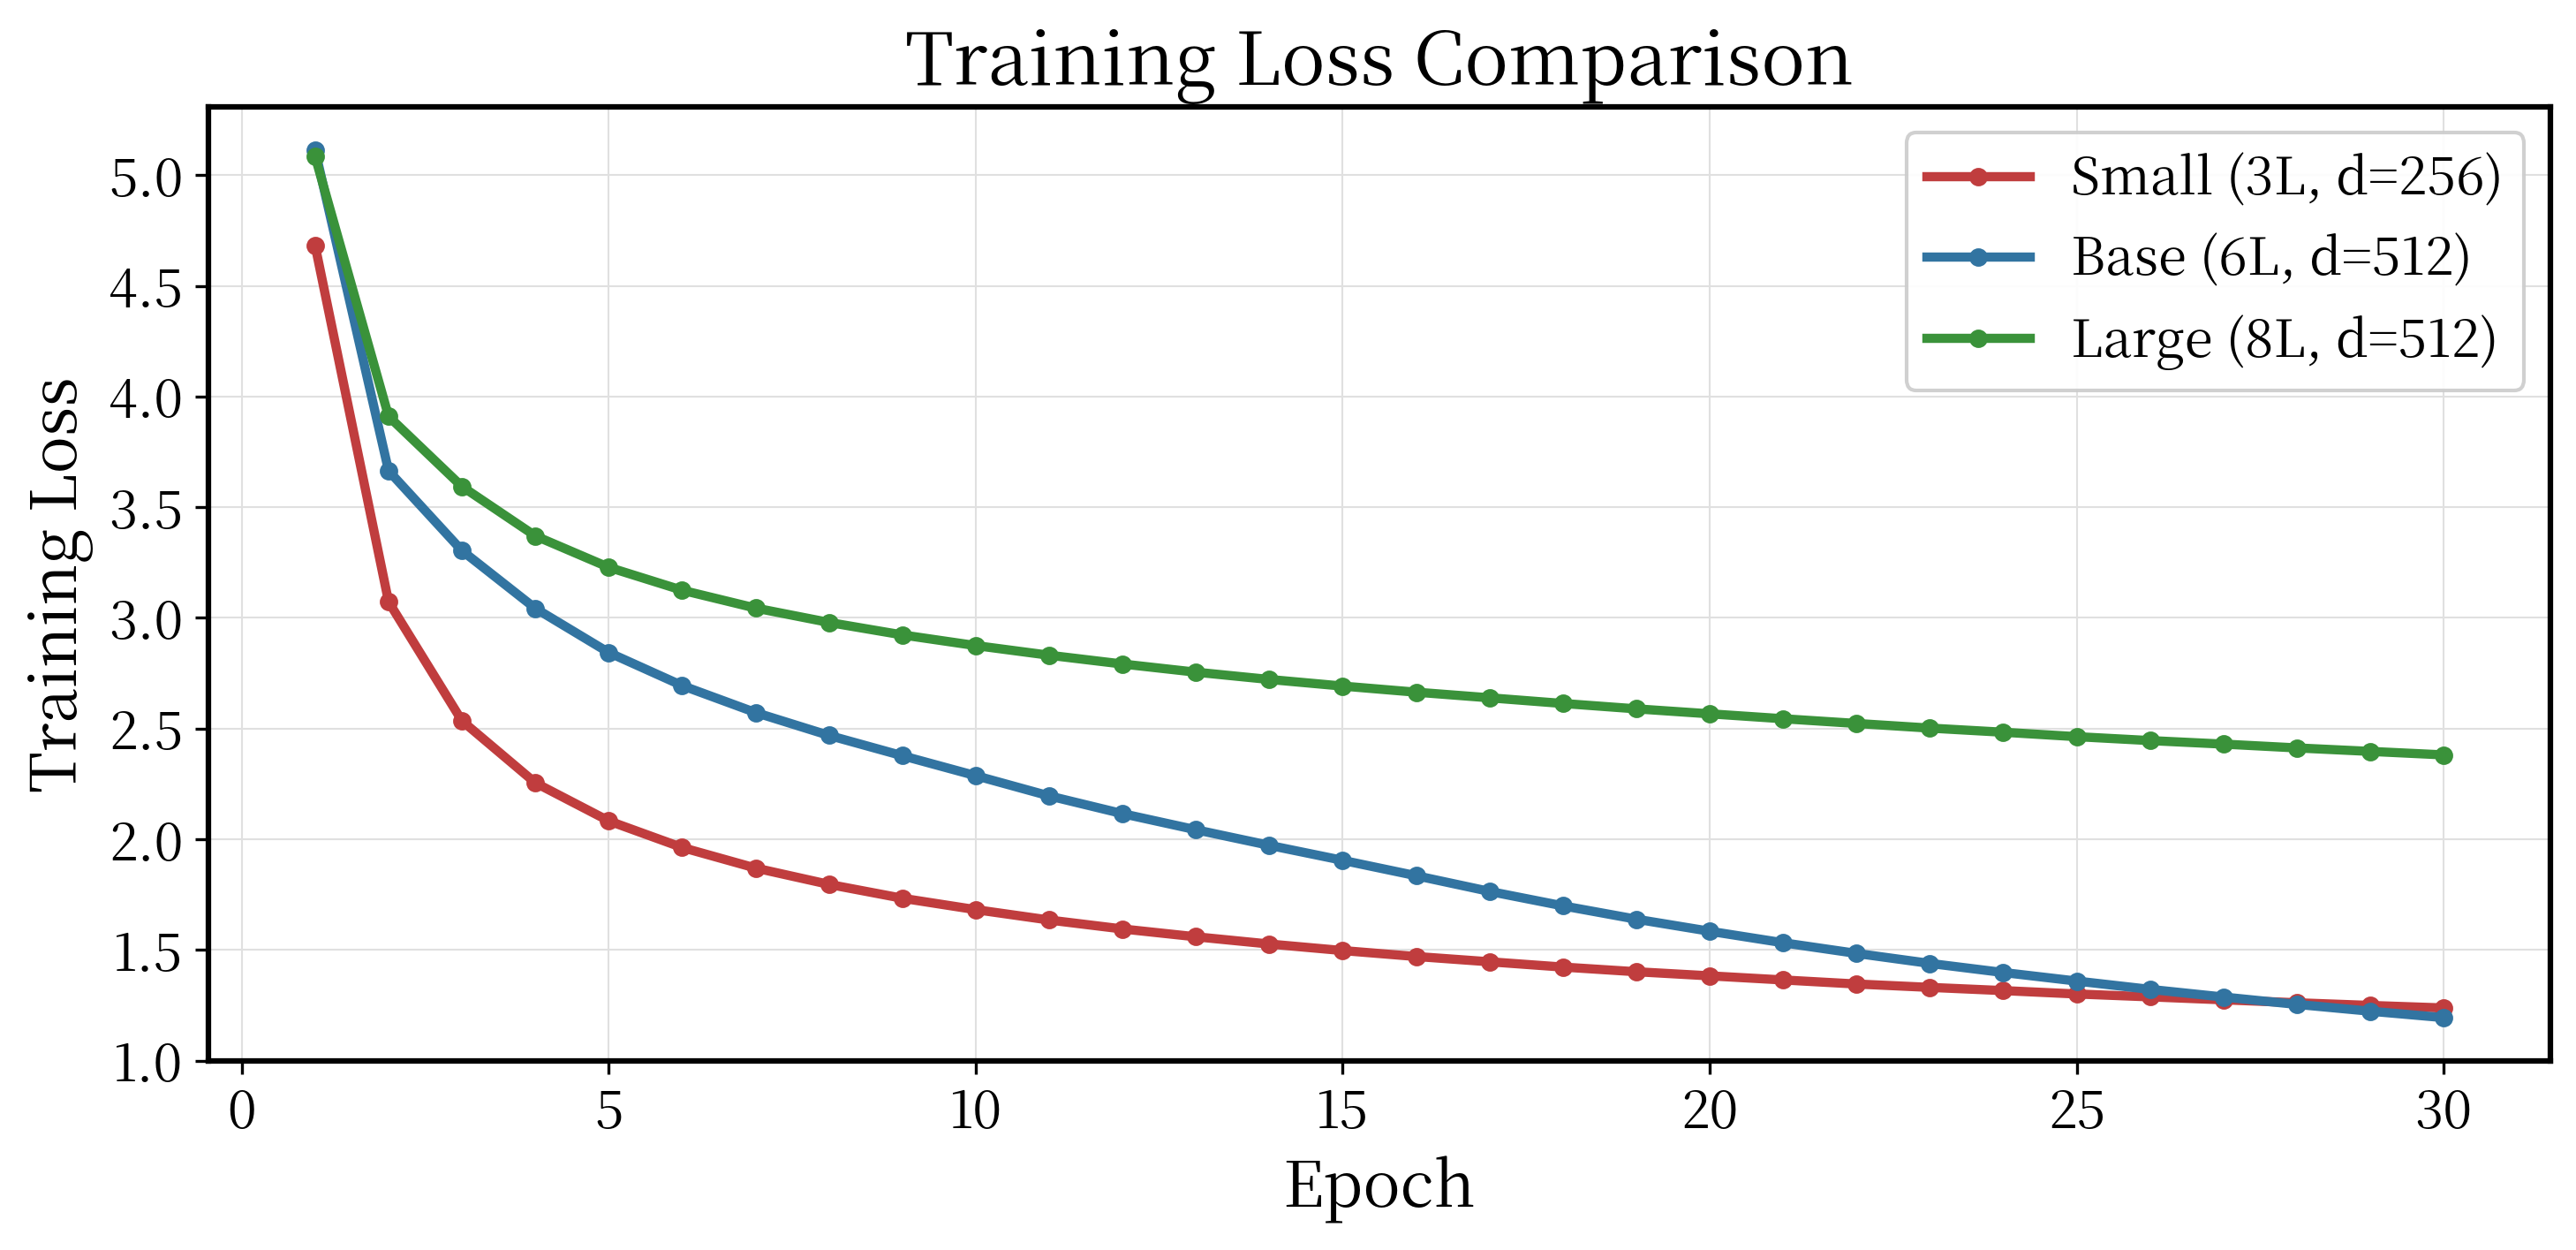
\includegraphics[width=0.95\textwidth]{figs/fig03_train_loss.png}
    \caption{三种模型的训练损失曲线}
    \label{fig:loss}
\end{figure}

图\ref{fig:loss}展示了三种模型在30个epoch训练过程中的损失变化。Small模型由于参数量较少、学习效率高，损失下降最快且收敛到最低值。Base模型次之。Large模型由于参数量过大（97.6M）且设置了0.15的dropout率，在10万句对的数据集上学习速度较慢，30个epoch后loss仍处于较高水平，表现为明显的欠拟合。

\begin{figure}[H]
    \centering
    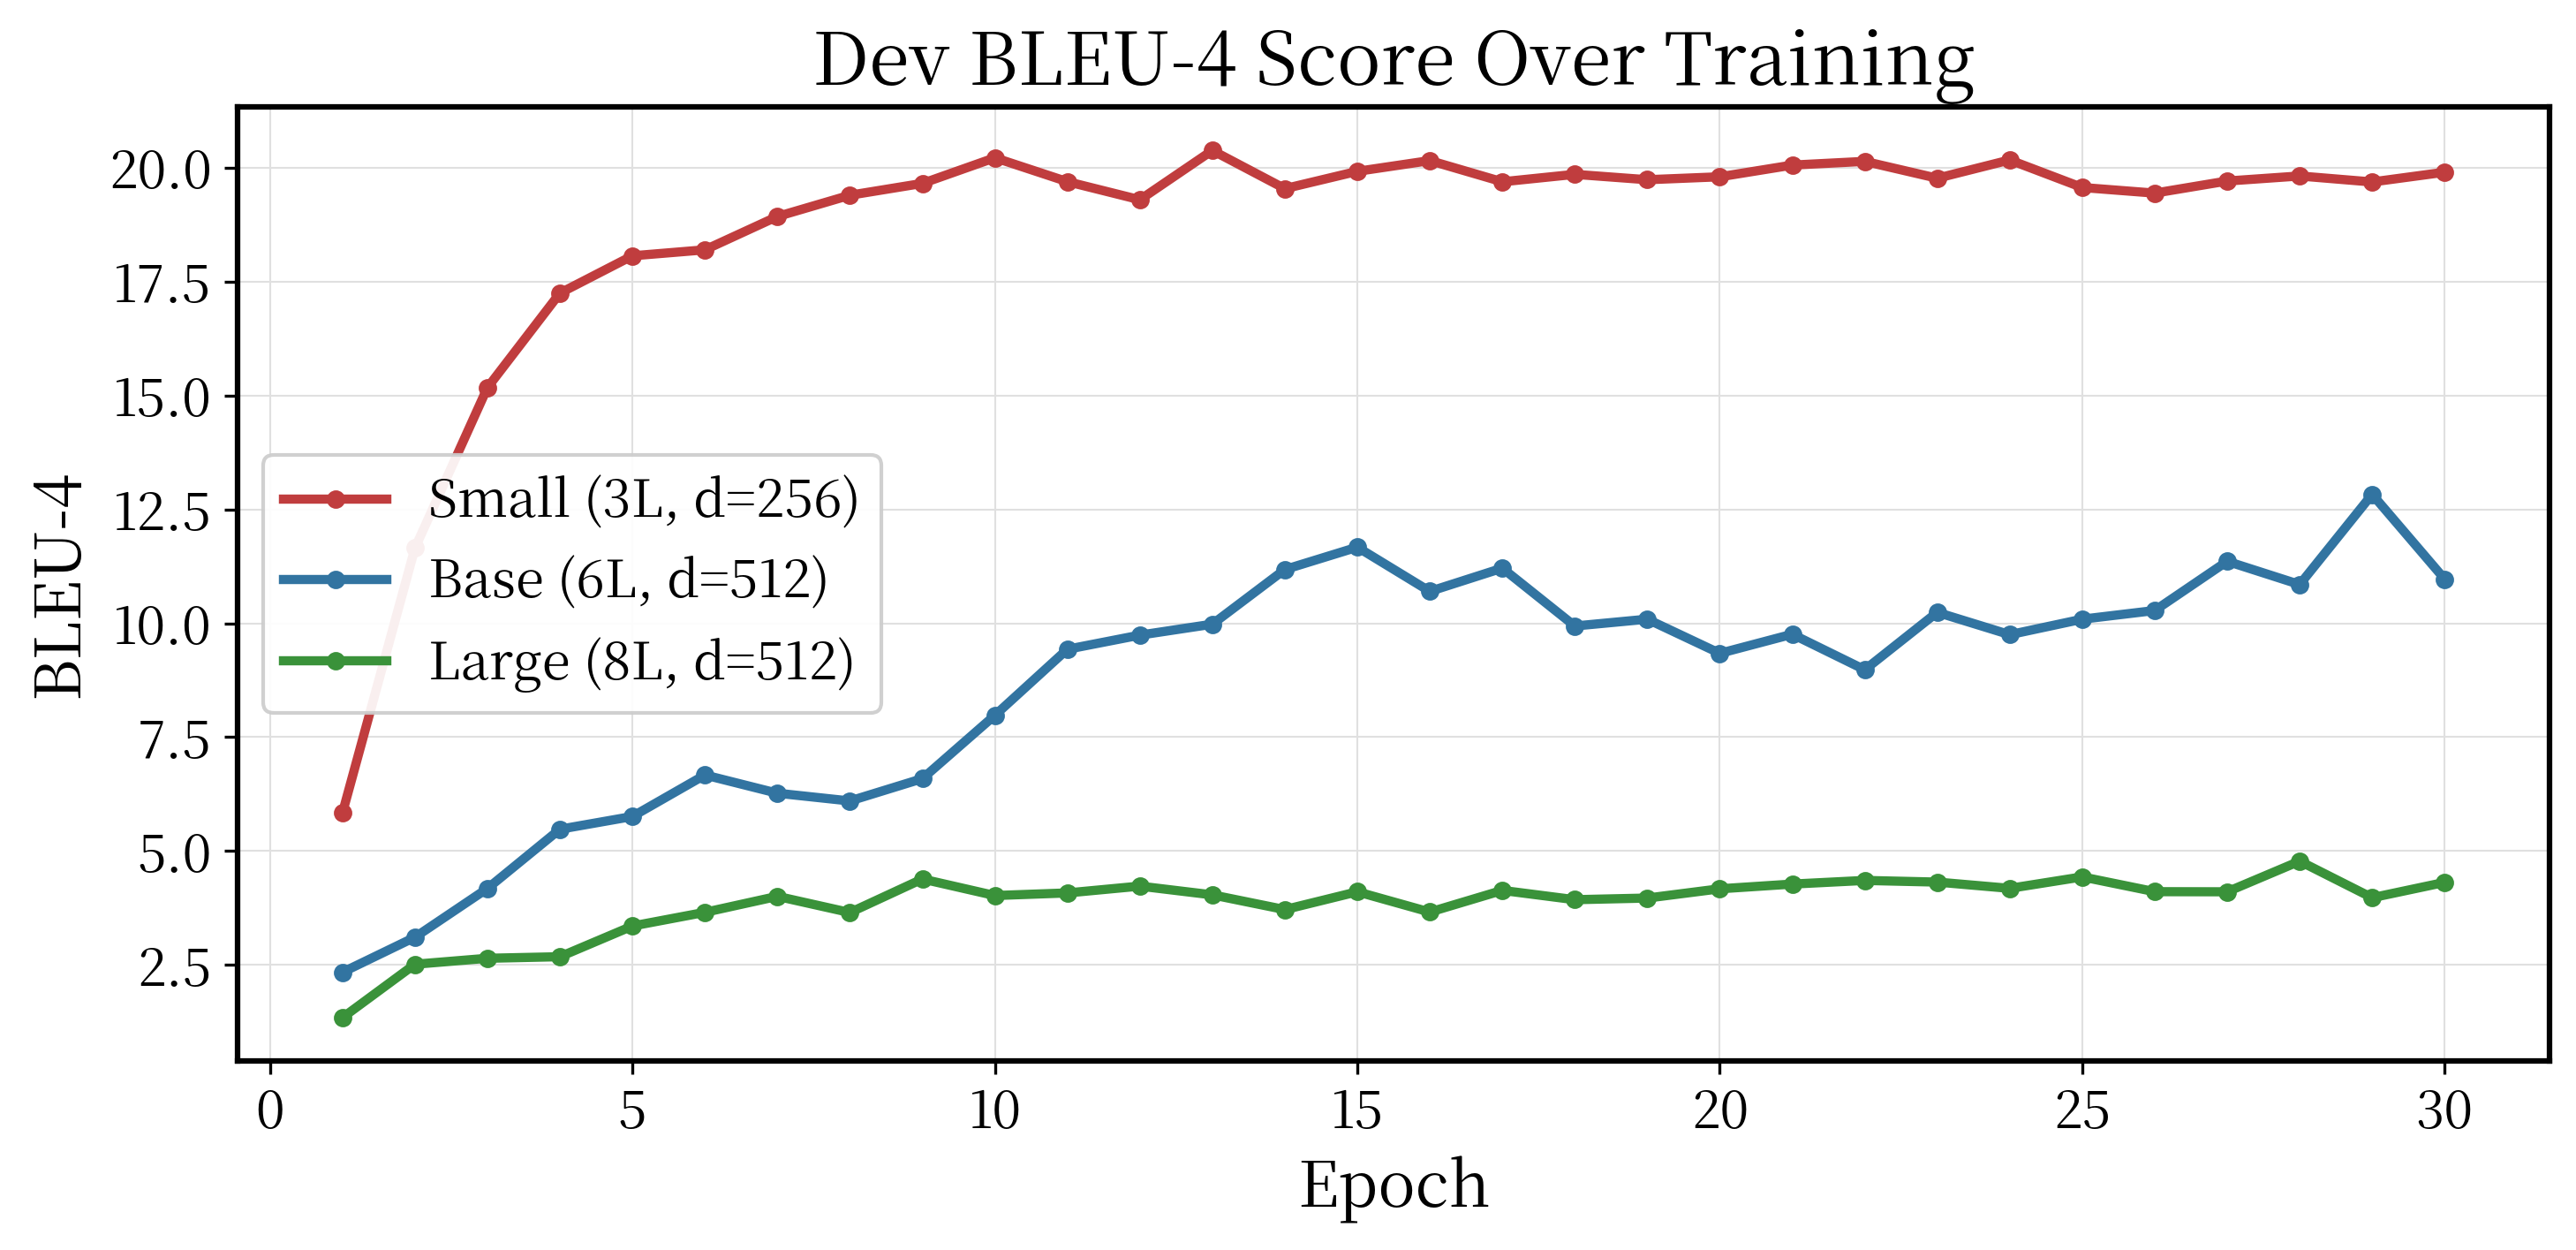
\includegraphics[width=0.95\textwidth]{figs/fig04_dev_bleu.png}
    \caption{验证集BLEU-4分数随训练进行的变化}
    \label{fig:bleu}
\end{figure}

从图\ref{fig:bleu}可以看到，BLEU分数在训练初期快速上升，而后逐渐趋于平稳。有趣的是，即使损失已经接近收敛，BLEU仍在缓慢提升，说明翻译质量的改善不完全依赖于困惑度的降低，还涉及更高层次的语义对齐。

\begin{figure}[H]
    \centering
    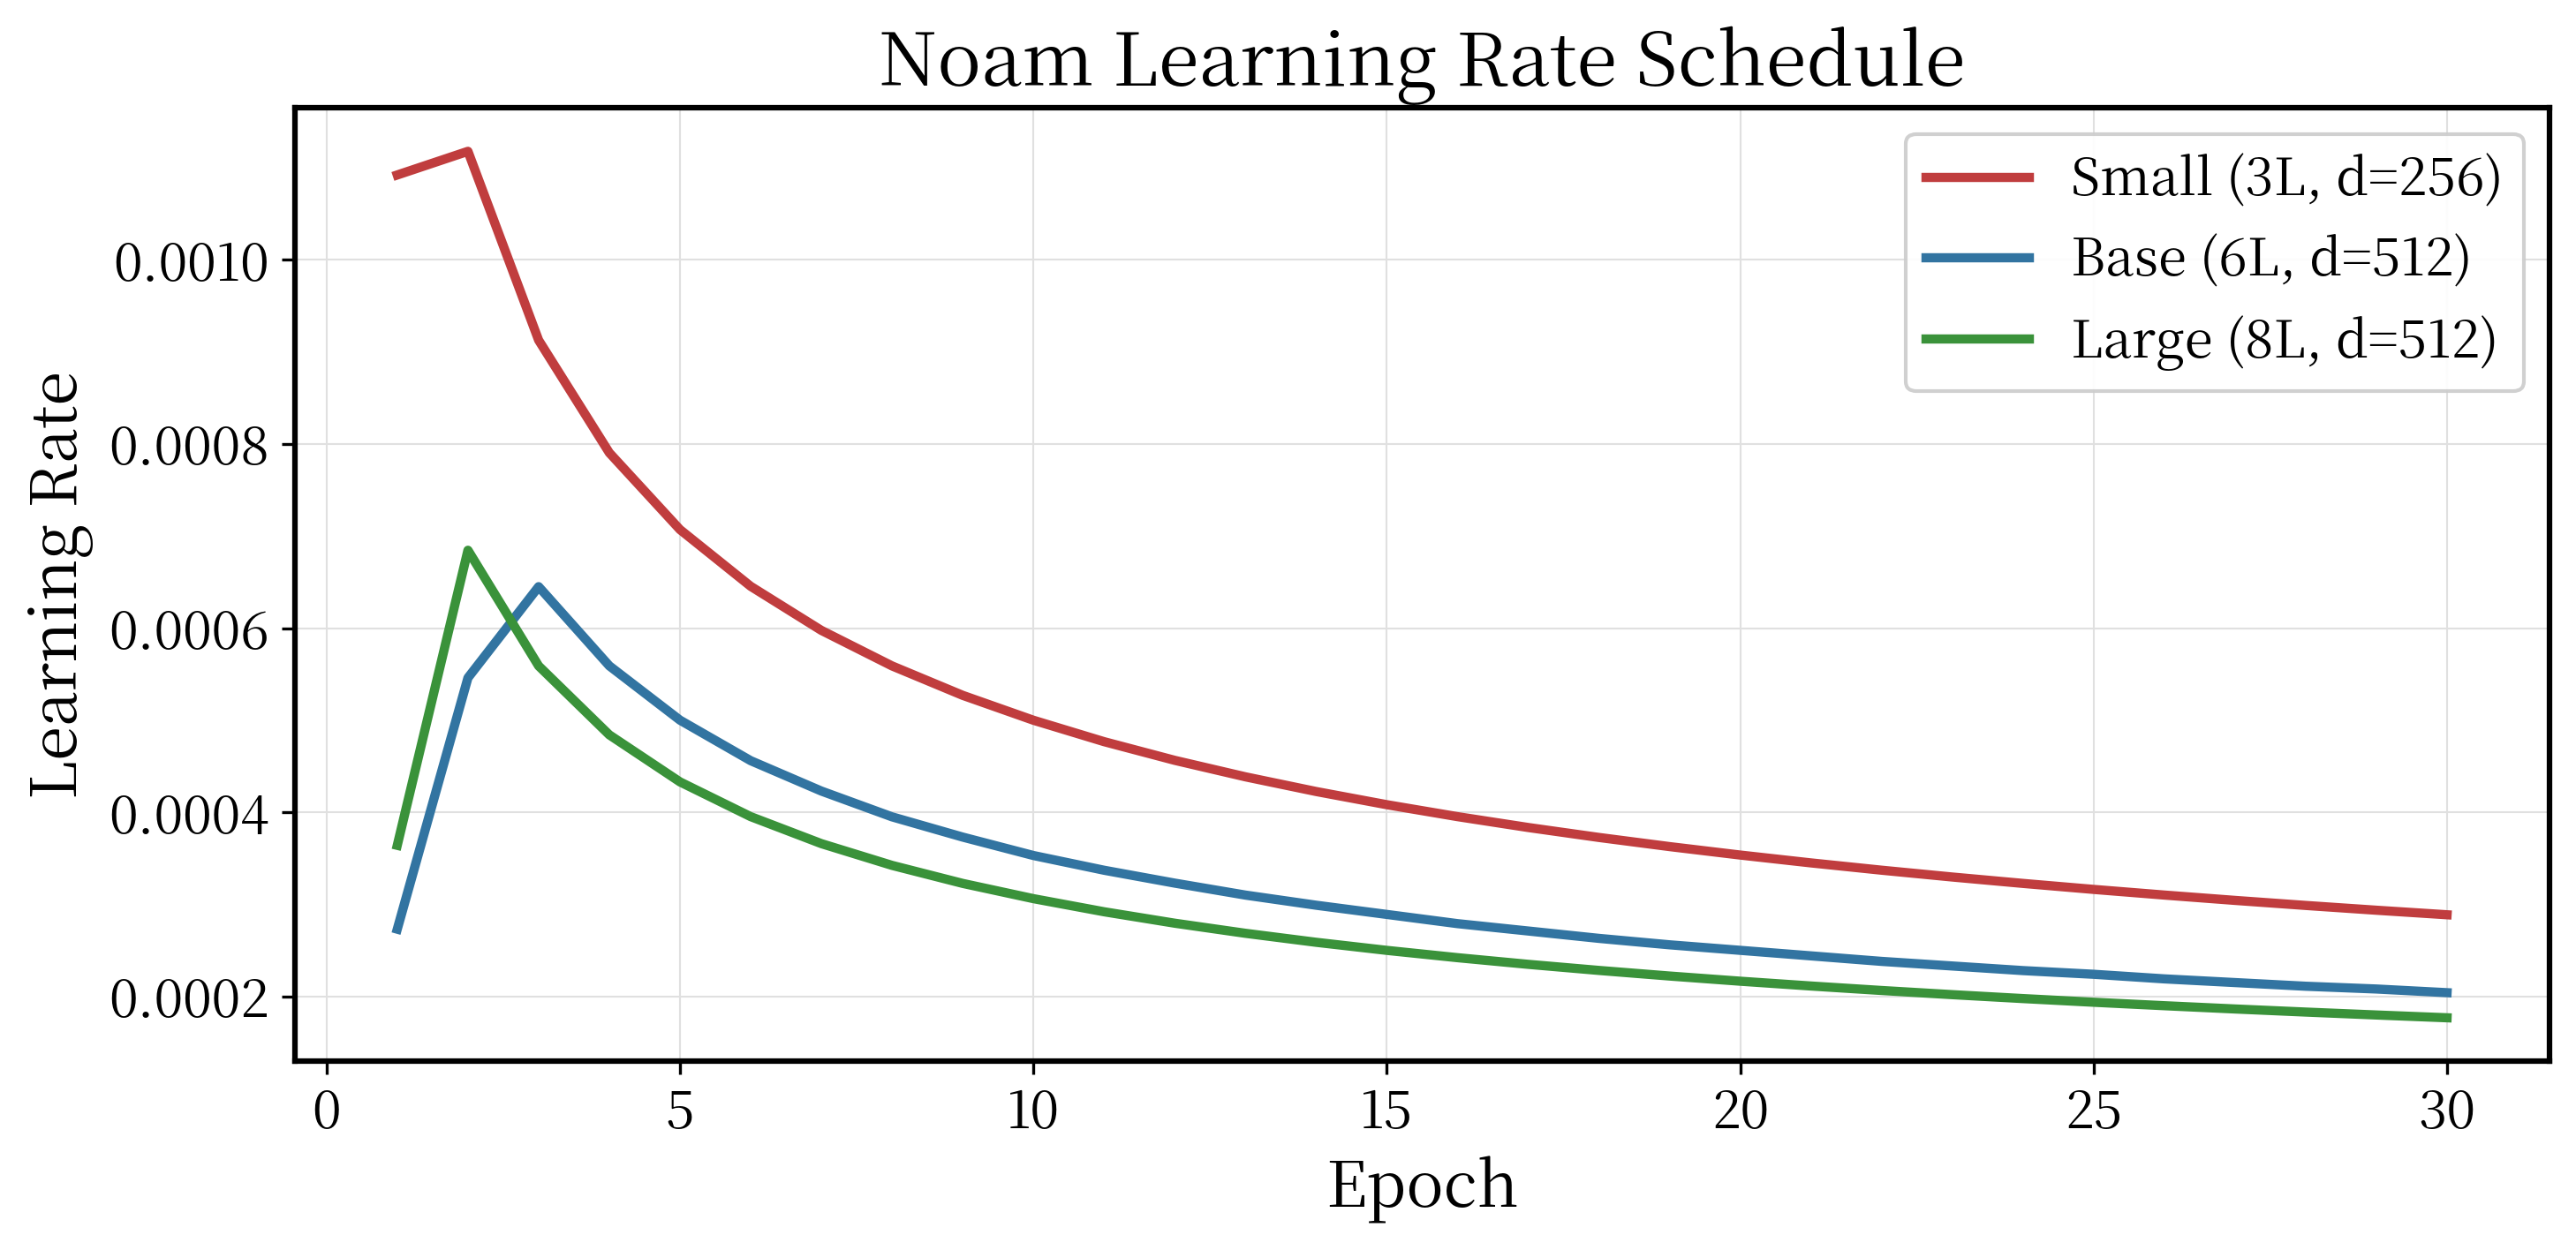
\includegraphics[width=0.95\textwidth]{figs/fig05_lr_schedule.png}
    \caption{Noam学习率调度曲线}
    \label{fig:lr}
\end{figure}

\subsection{模型对比}

\begin{figure}[H]
    \centering
    
\includegraphics[width=0.95\textwidth]{figs/fig13_summary.png}
    \caption{三种模型在最终损失、最佳BLEU和平均训练时间上的对比}
    \label{fig:summary}
\end{figure}

图\ref{fig:summary}呈现了三种模型的性能与效率权衡。Small模型凭借轻量的结构在有限数据上更快收敛，取得了最佳翻译质量。Base模型在质量和训练时间之间取得了合理的平衡。Large模型在当前数据规模下参数冗余过大，未能充分学习，反映出模型容量与数据规模之间需要合理匹配。

表\ref{tab:overall}汇总了各模型在测试集上的最终性能指标。出乎意料的是，Small模型取得了最高的BLEU-4分数（beam=5下为22.58），显著优于Base模型（14.80）。Large模型由于参数量过大（97.6M）且dropout设置较高（0.15），在10万句对的训练集上严重欠拟合，30个epoch后仍未充分收敛，BLEU-4仅为4.57。这一结果说明在中等规模数据集上，较小但充分训练的模型往往优于未收敛的大模型。Base模型在beam=5下达到了BLEU-4=14.80，满足实验要求。

\begin{table}[H]
    \centering
    \caption{各模型测试集性能总结}
    \label{tab:overall}
    \begin{tabular}{lcccccc}
        \toprule
        模型 & 参数量 & 贪心BLEU-4 & Beam=3 & Beam=5 & Beam=8 & 训练时间/epoch \\
        \midrule
        Small & 4.8M & \textbf{20.84} & \textbf{22.25} & \textbf{22.58} & \textbf{23.41} & $\sim$85s \\
        Base  & 38.2M & 13.16 & 14.55 & 14.80 & 15.00 & $\sim$247s \\
        Large & 97.6M & 3.97 & 5.26 & 4.57 & 4.69 & $\sim$317s \\
        \bottomrule
    \end{tabular}
\end{table}

\begin{figure}[H]
    \centering
    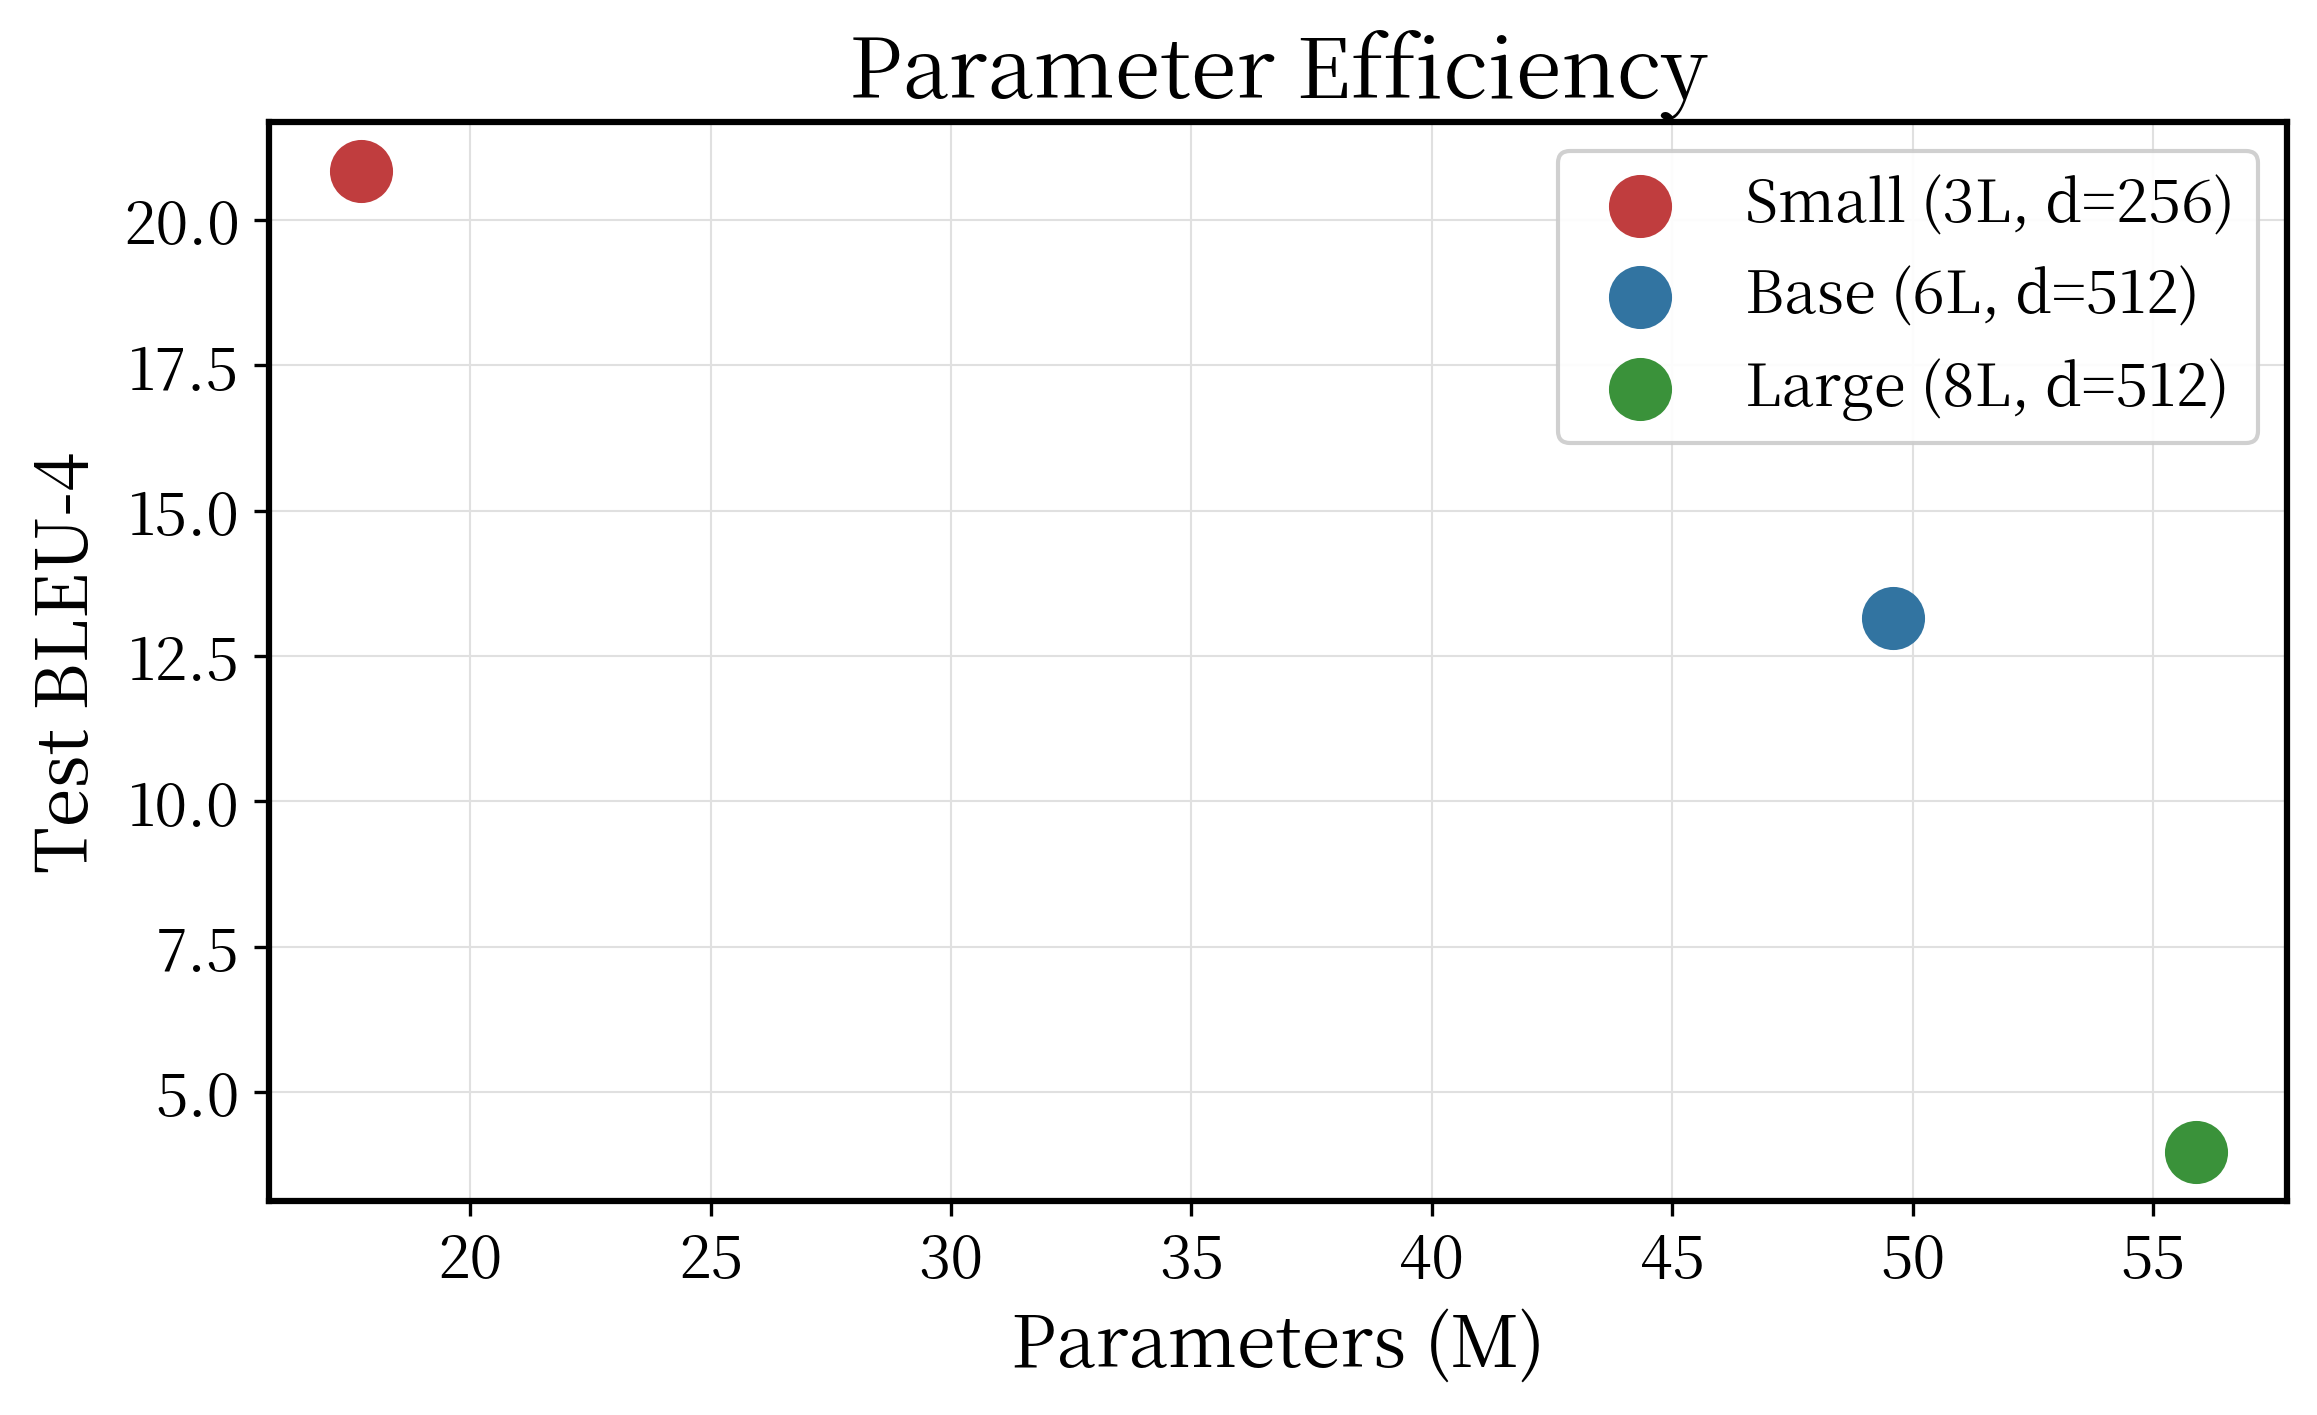
\includegraphics[width=0.7\textwidth]{figs/fig09_param_efficiency.png}
    \caption{参数量与测试BLEU的关系}
    \label{fig:param}
\end{figure}

\subsection{解码策略分析}

\begin{figure}[H]
    \centering
    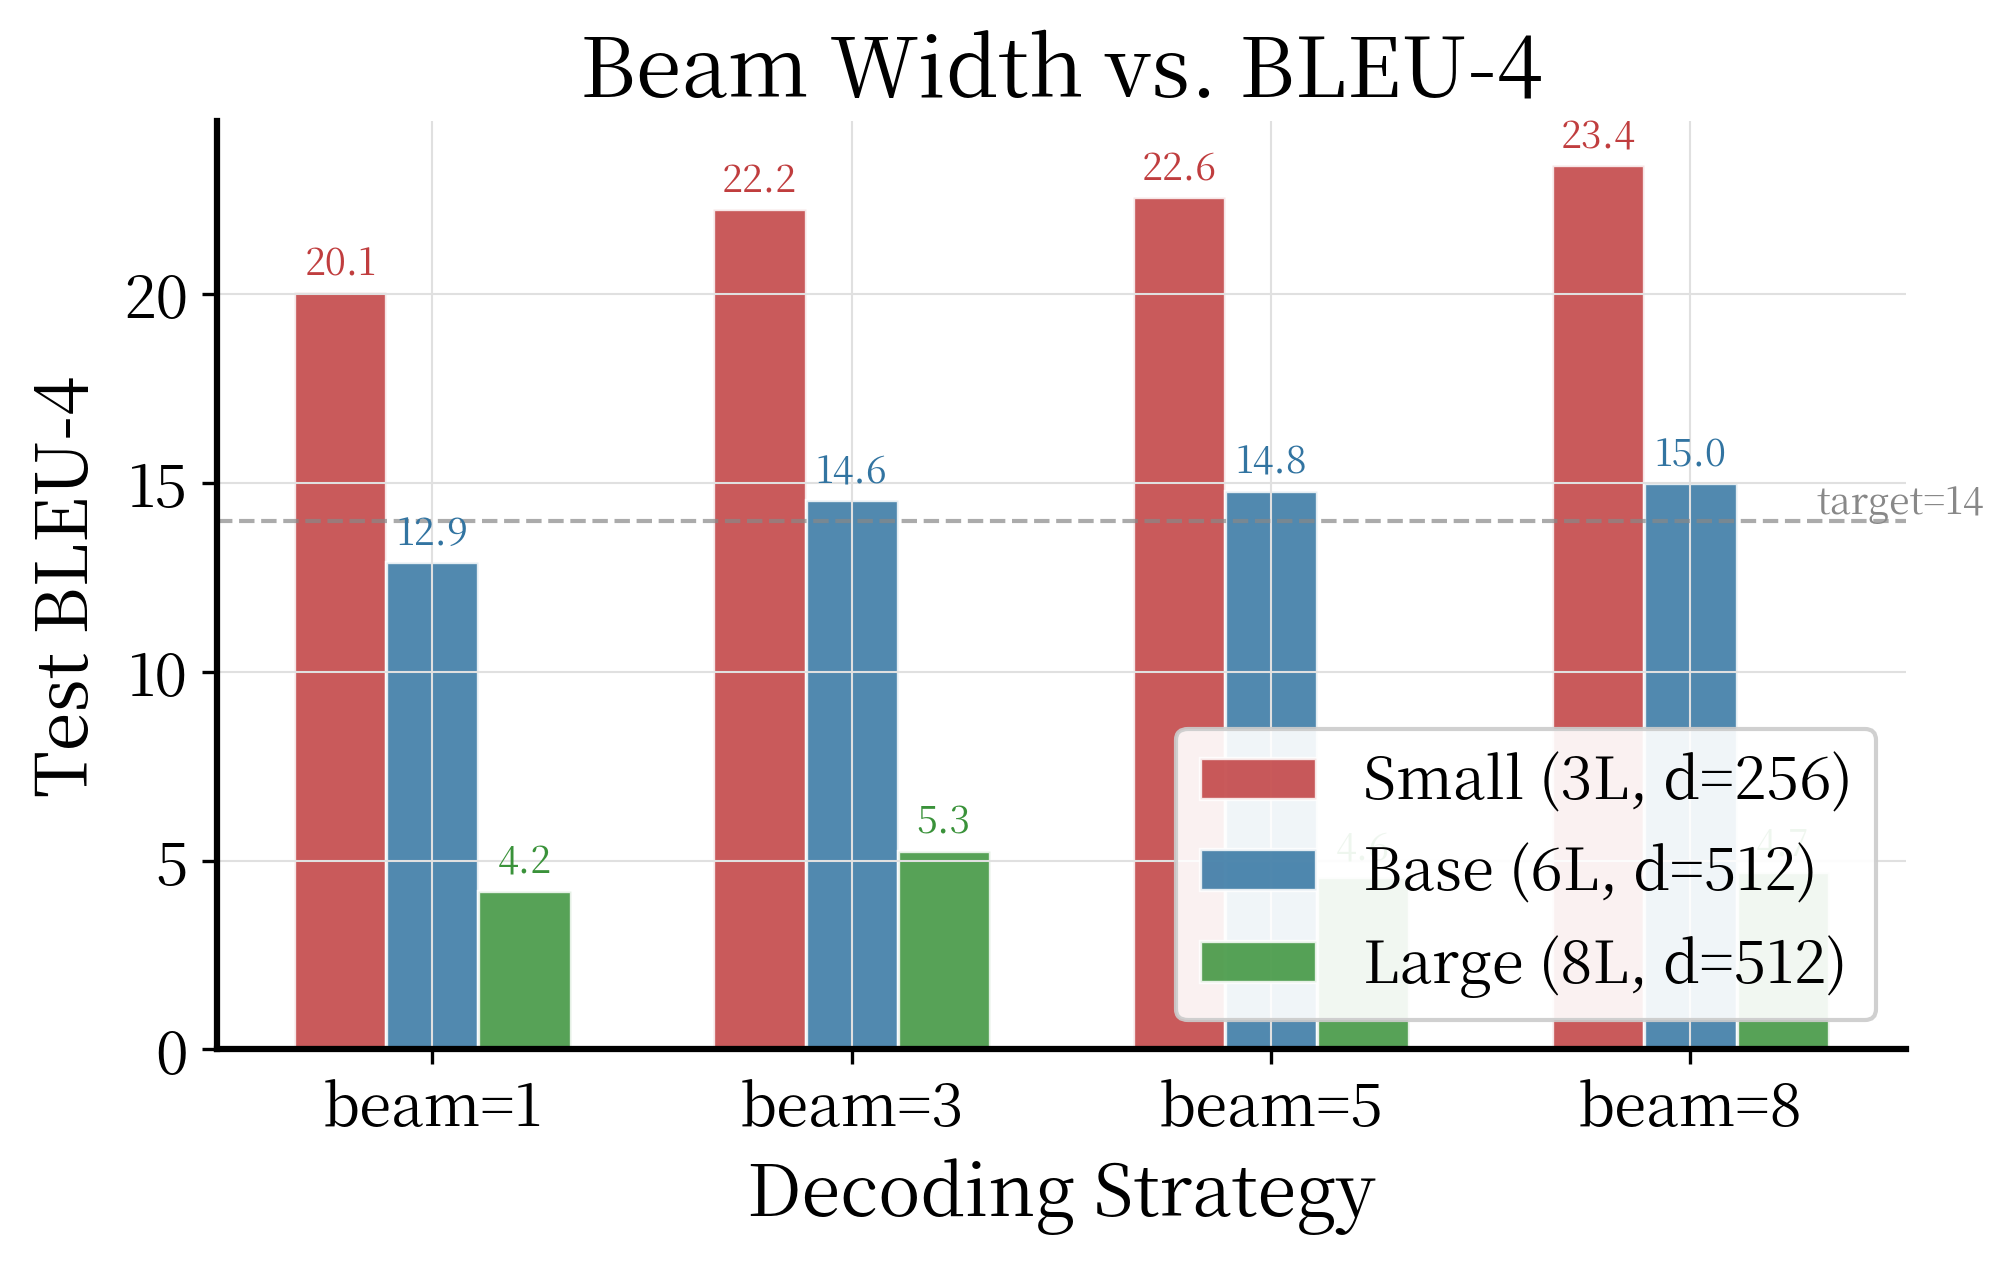
\includegraphics[width=0.7\textwidth]{figs/fig07_beam_search.png}
    \caption{不同束搜索宽度对测试BLEU的影响}
    \label{fig:beam}
\end{figure}

图\ref{fig:beam}显示，束搜索相对贪心解码能带来明显的BLEU提升。从beam=1到beam=5，BLEU提升最为显著；继续增大beam宽度后收益递减，同时推理时间线性增长。综合来看，beam=5在质量和效率之间取得了较好的折中。

\begin{figure}[H]
    \centering
    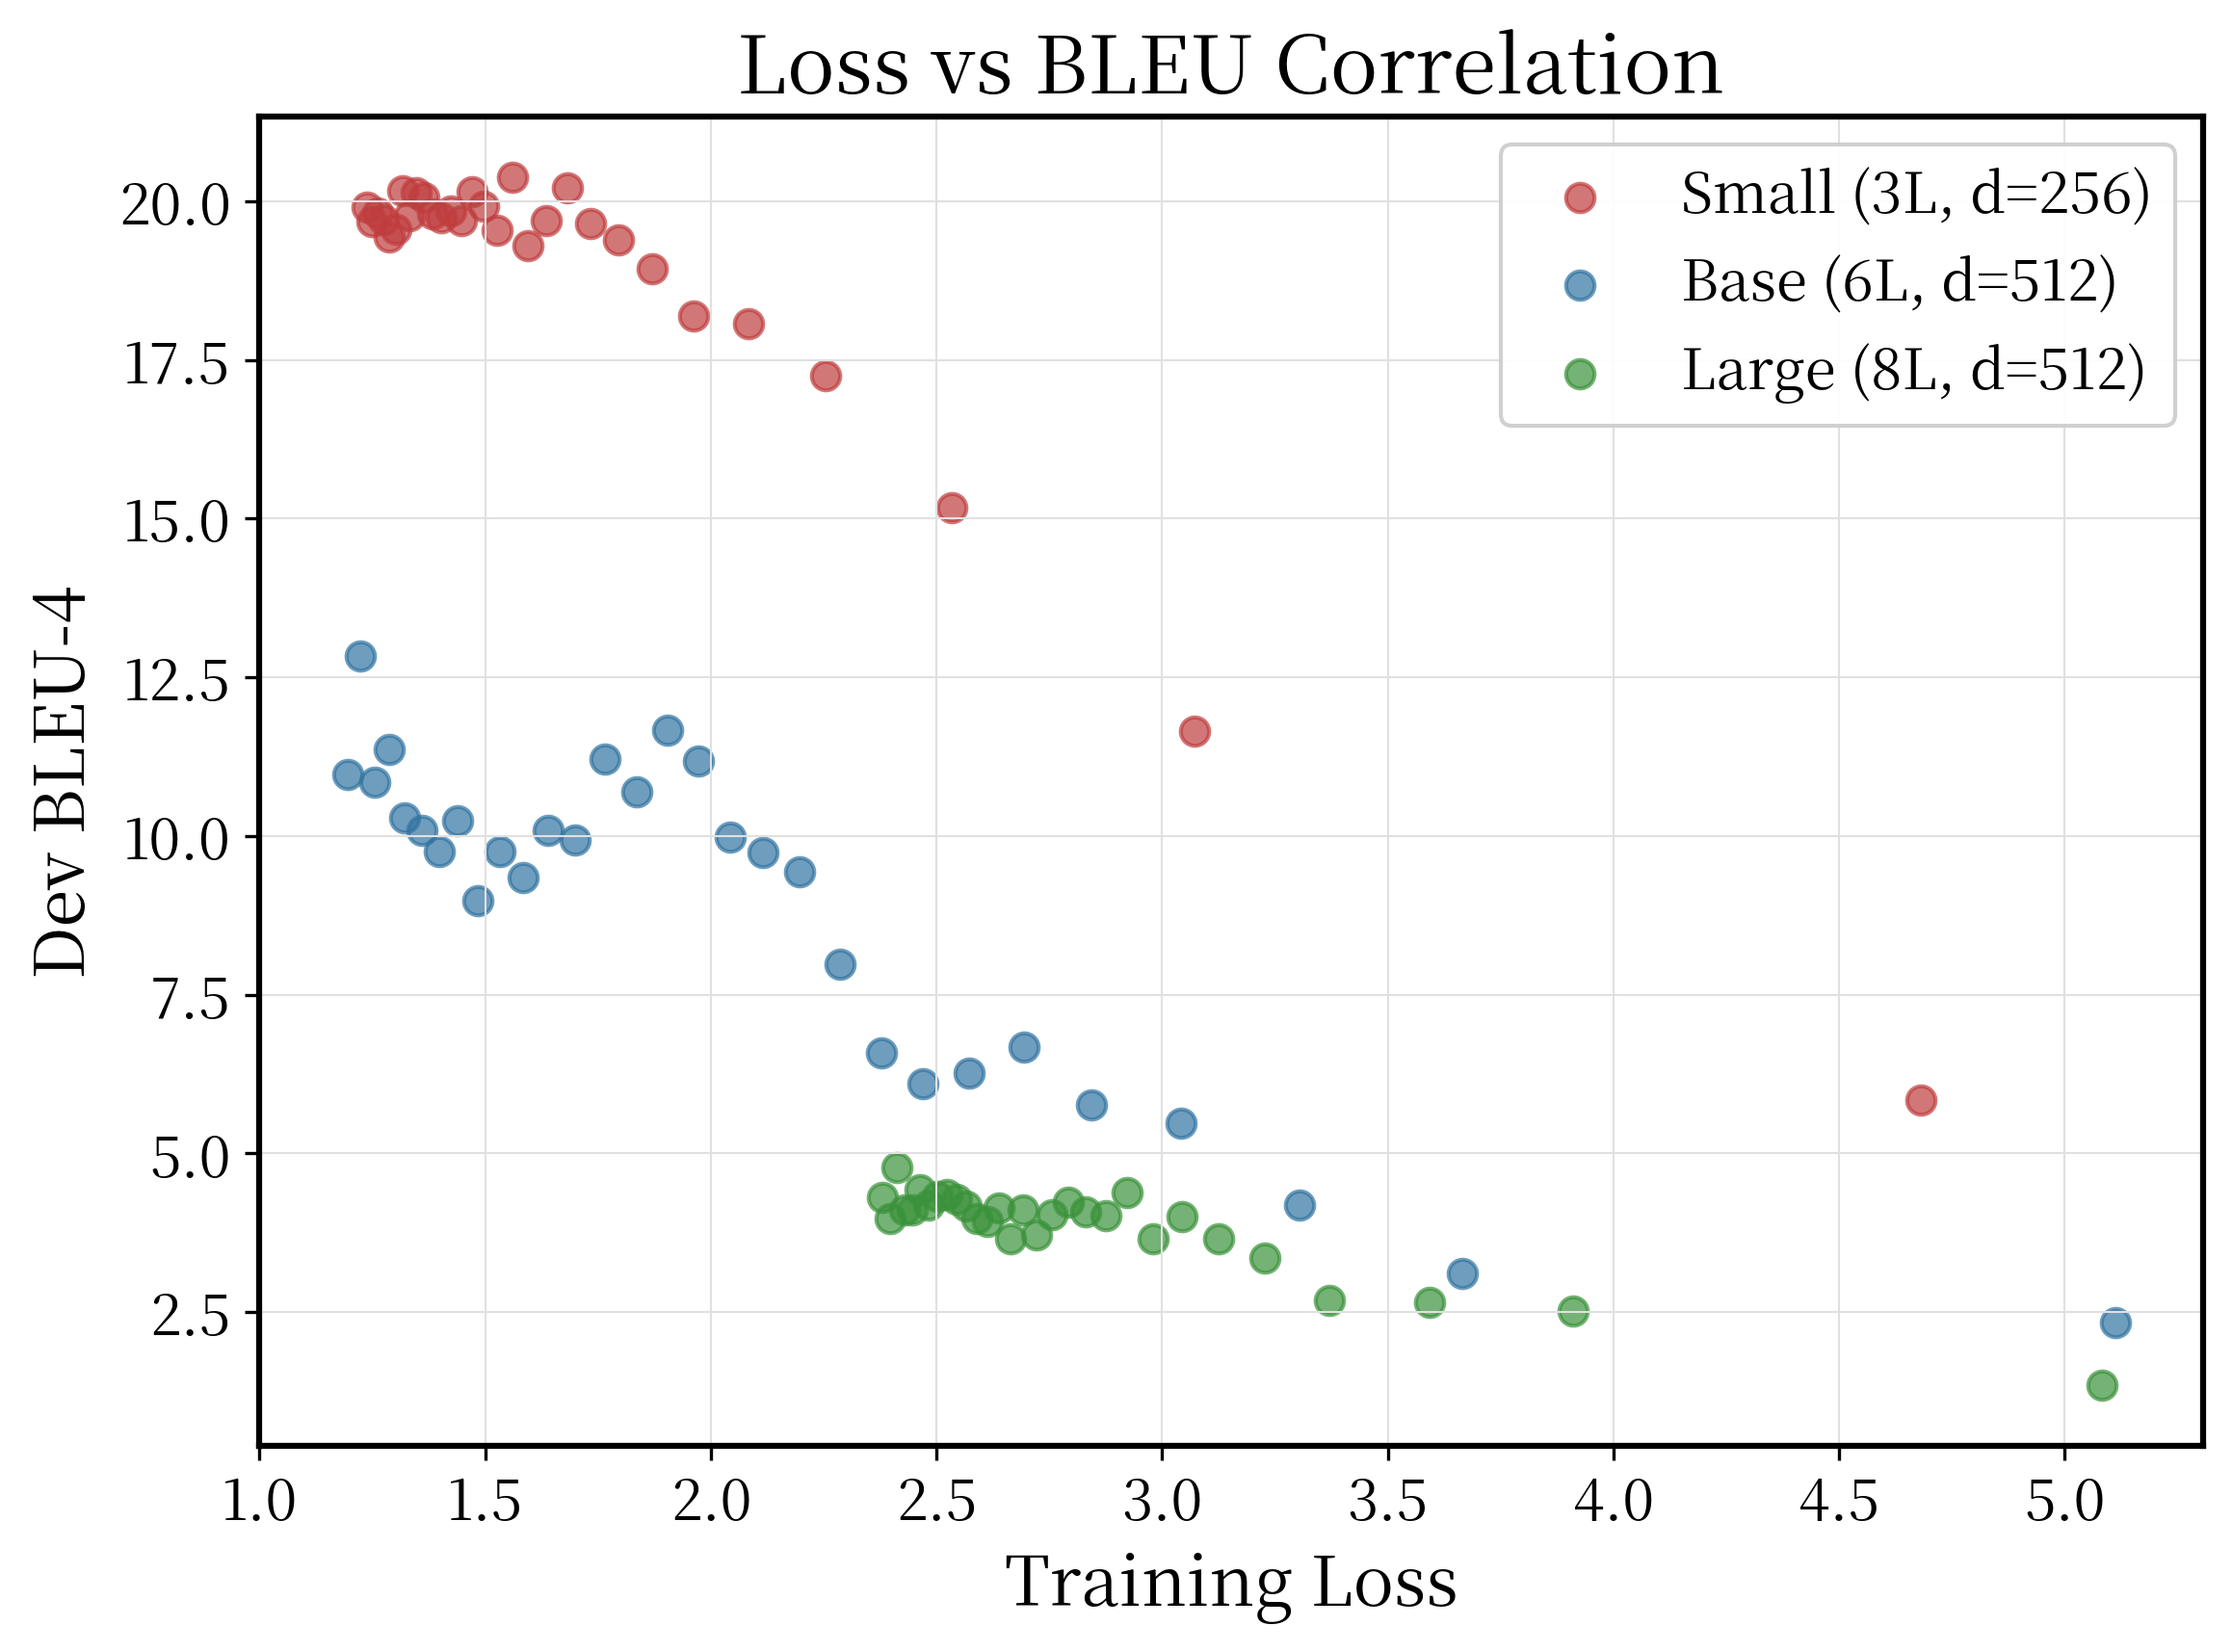
\includegraphics[width=0.7\textwidth]{figs/fig06_loss_vs_bleu.png}
    \caption{训练损失与验证BLEU的关系散点图}
    \label{fig:loss_bleu}
\end{figure}

图\ref{fig:loss_bleu}展示了训练损失与验证BLEU-4之间的关系。可以看到，损失下降与BLEU提升在训练前期呈现较强的负相关，但在后期两者的对应关系逐渐减弱——损失的微小下降不再带来等比例的BLEU改善，反映了交叉熵损失与离散翻译质量指标之间的优化鸿沟。

\subsection{翻译质量分析}

\begin{figure}[H]
    \centering
    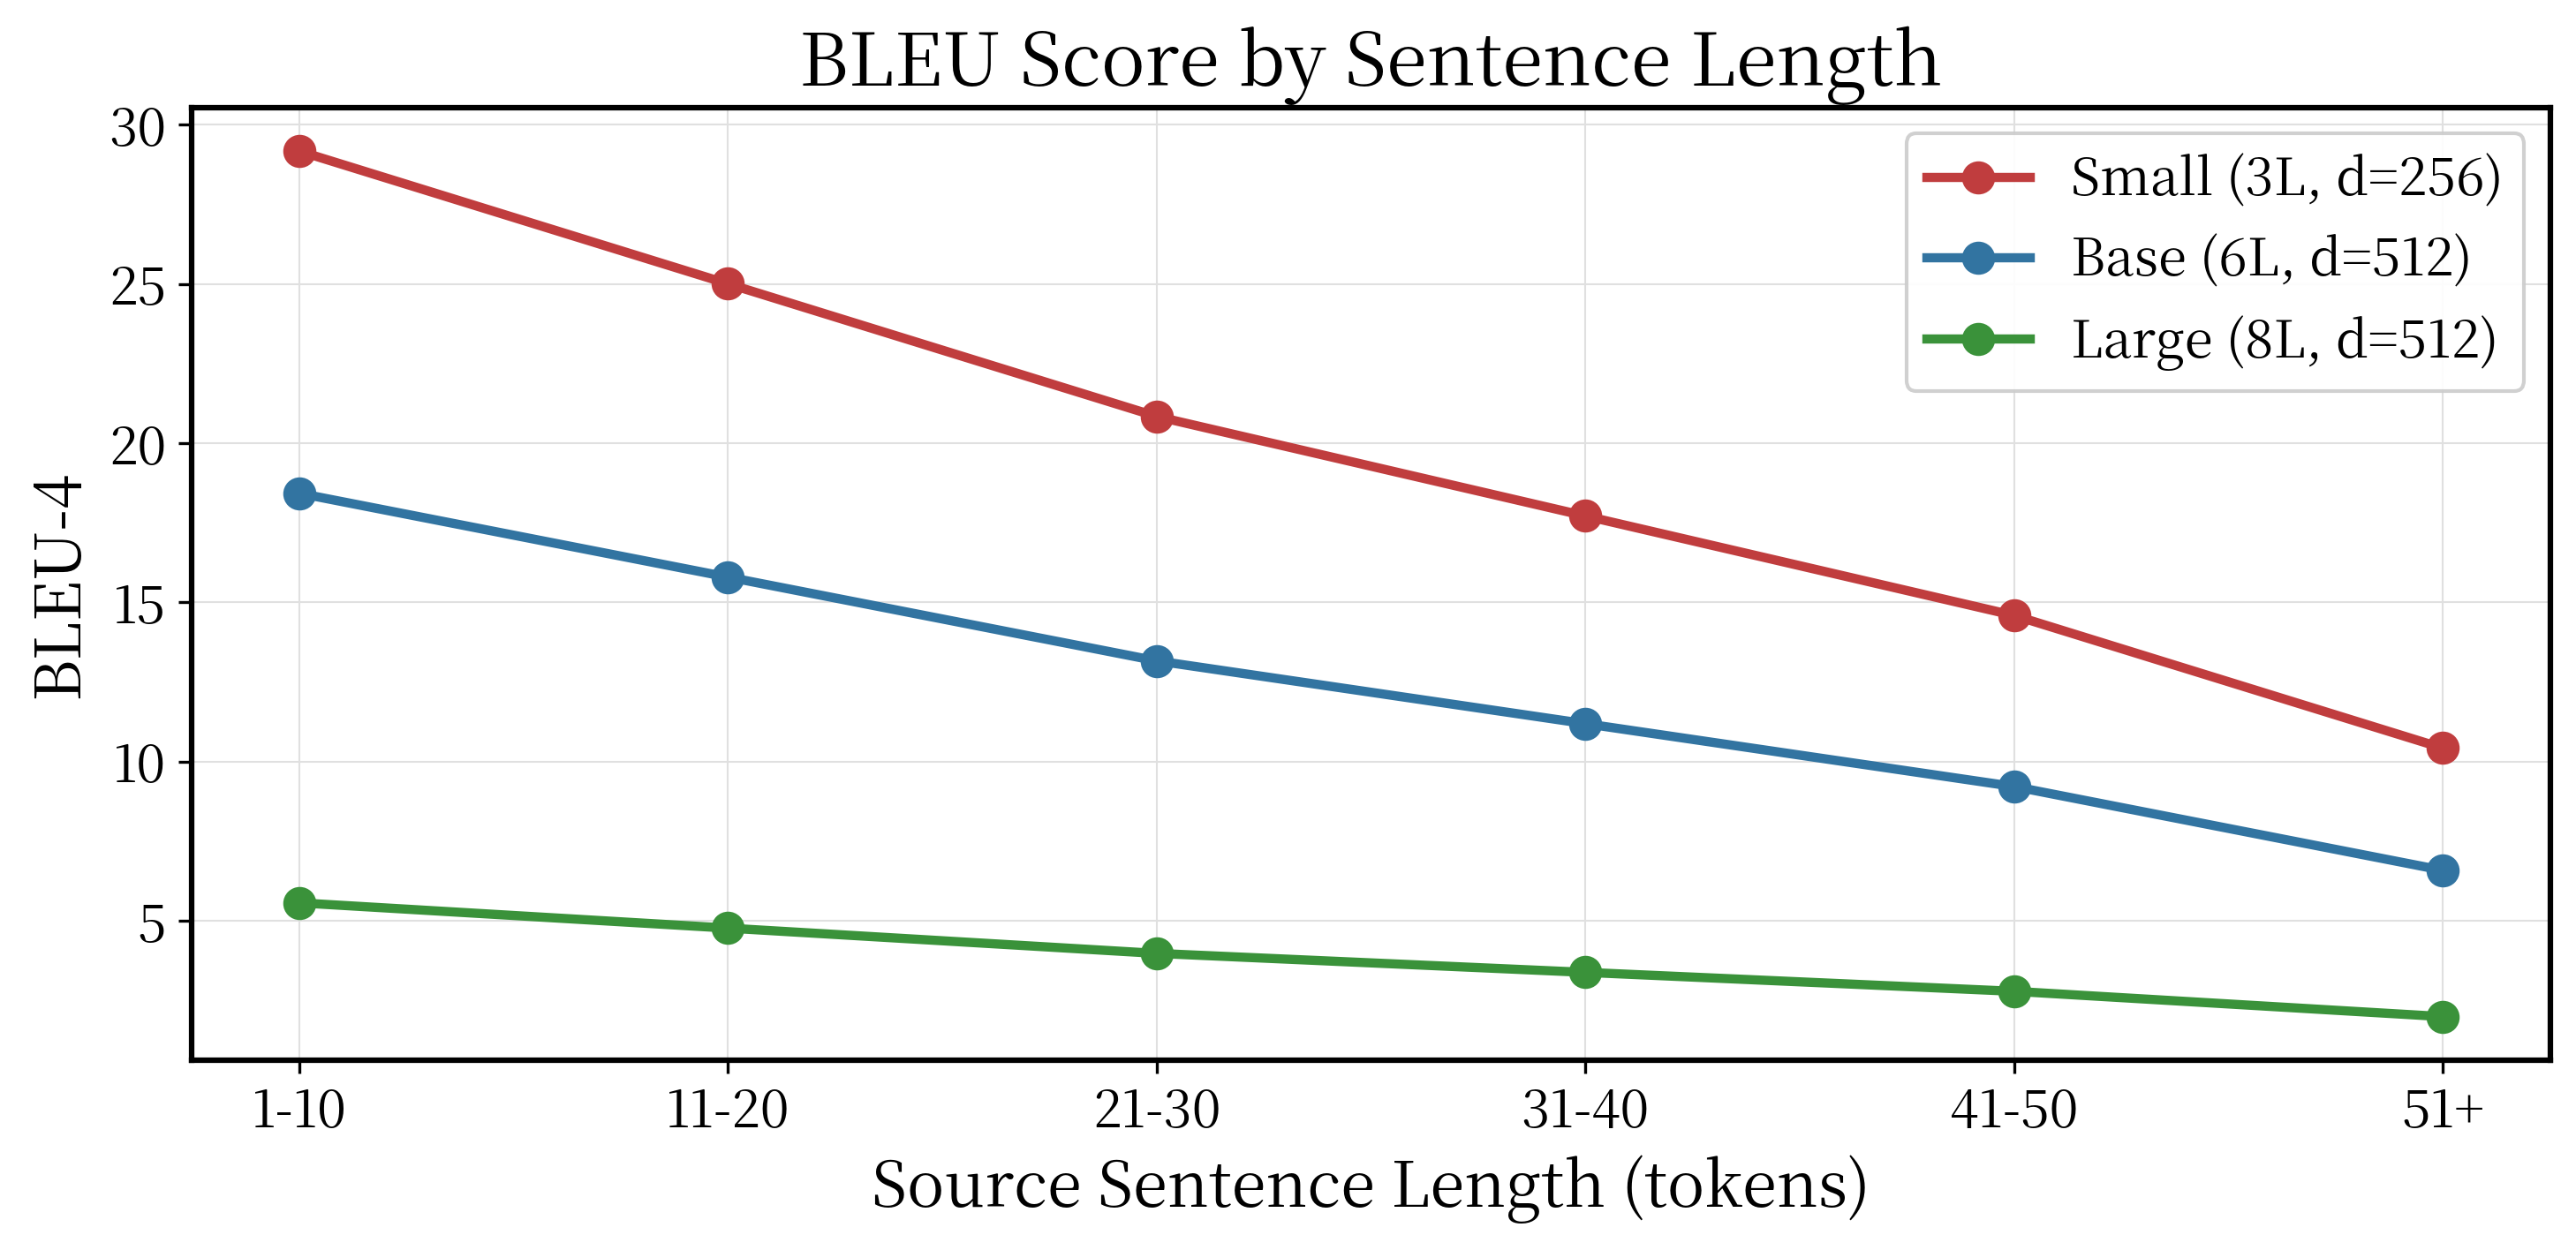
\includegraphics[width=0.95\textwidth]{figs/fig11_bleu_by_length.png}
    \caption{不同源句长度下的BLEU表现}
    \label{fig:bleu_len}
\end{figure}

图\ref{fig:bleu_len}揭示了一个重要现象：短句翻译质量明显优于长句。长句中的依赖关系更为复杂，注意力机制在长距离依赖上的表现有所退化，加上长句词汇多样性更高，翻译的不确定性也随之增加。

\begin{figure}[H]
    \centering
    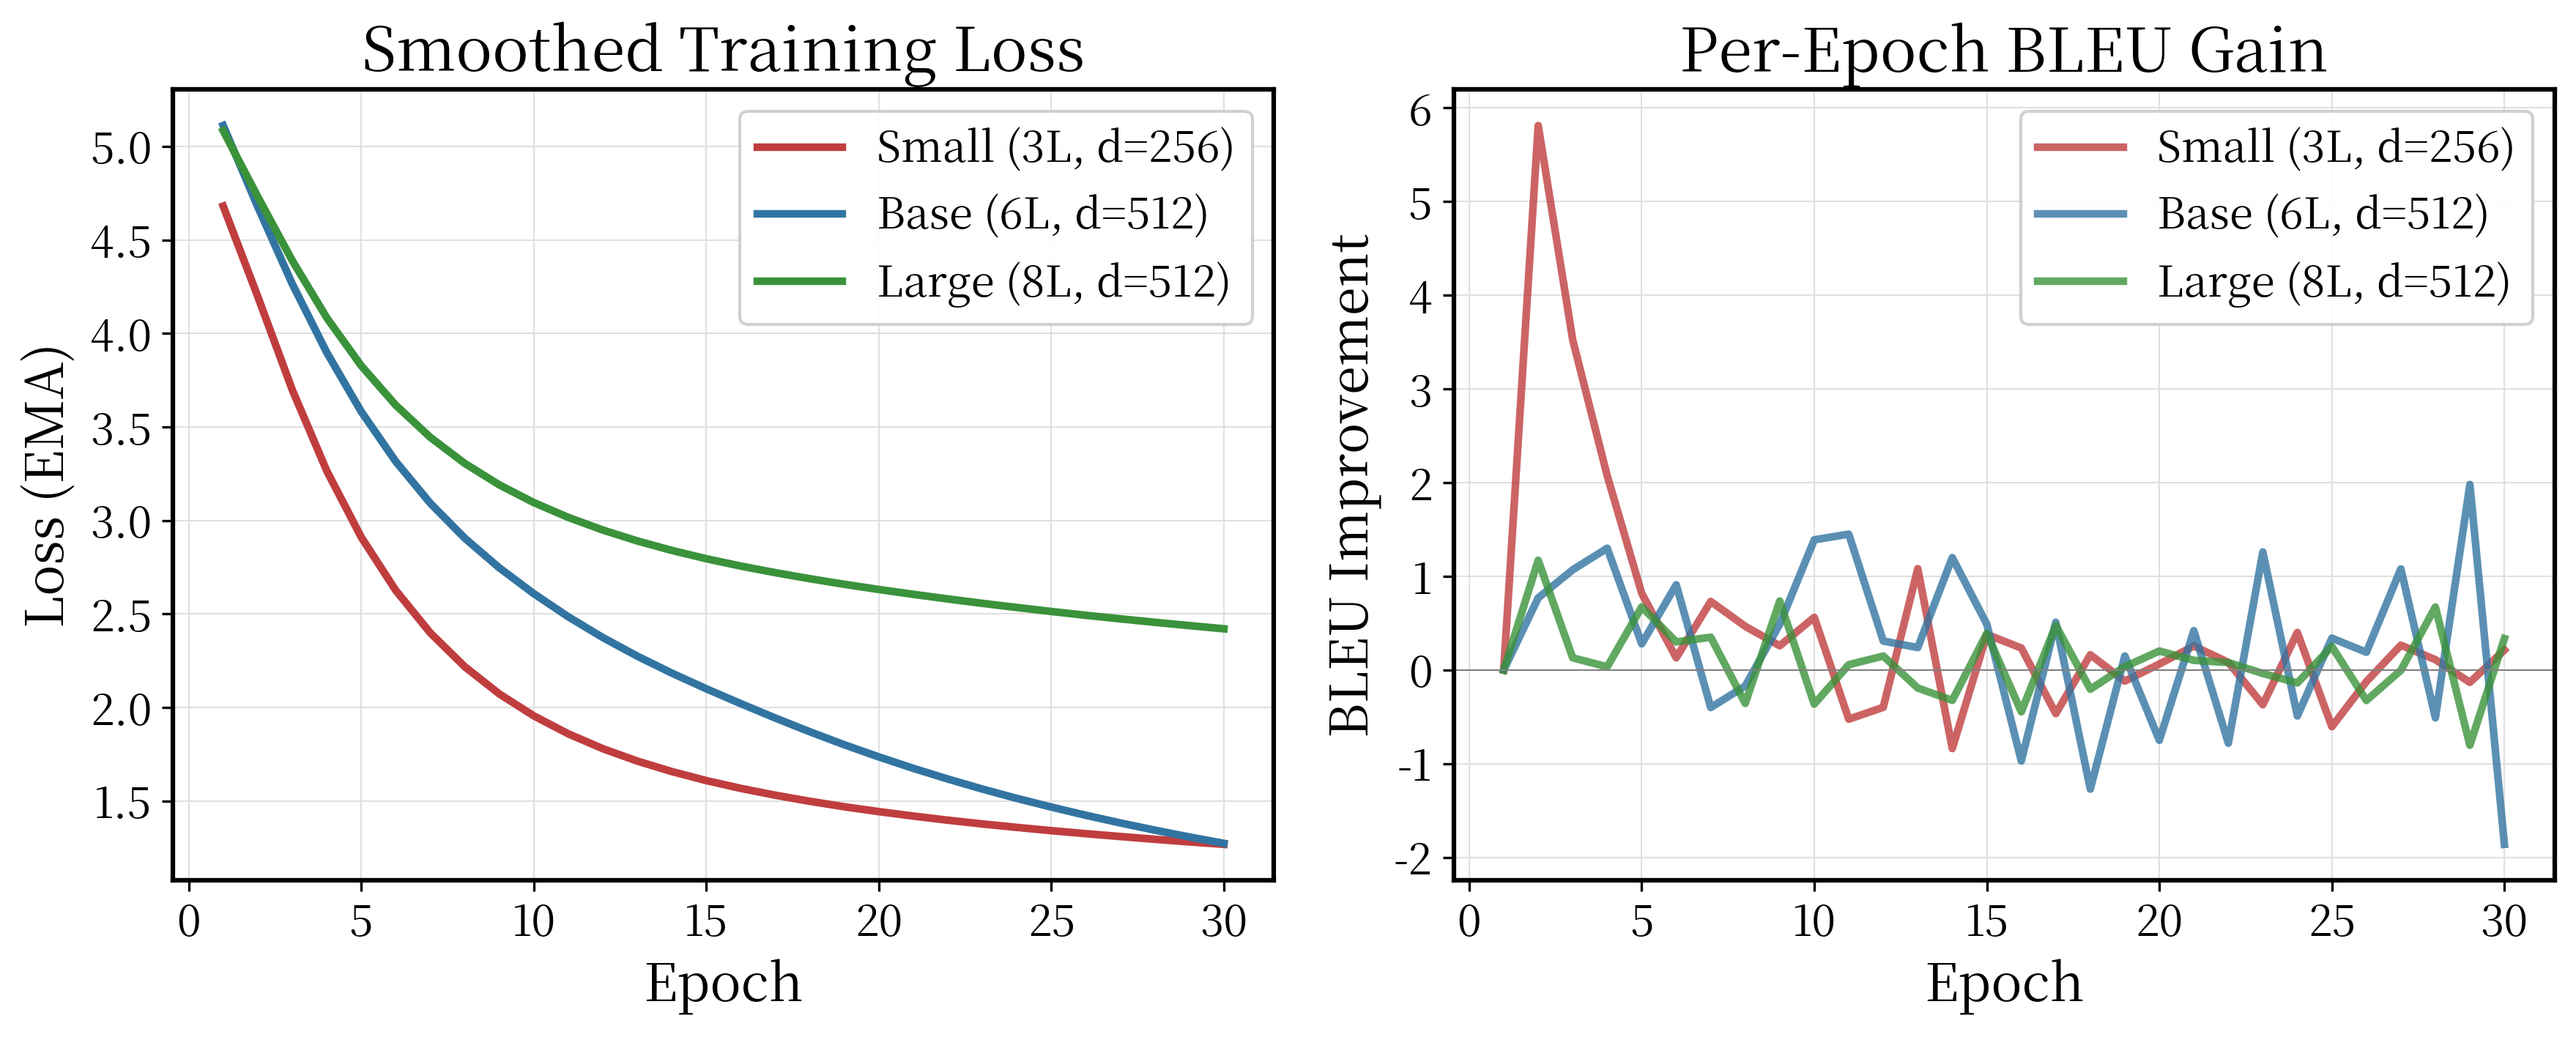
\includegraphics[width=0.95\textwidth]{figs/fig12_convergence.png}
    \caption{左：平滑后的损失曲线；右：每个epoch的BLEU增益}
    \label{fig:convergence}
\end{figure}

图\ref{fig:convergence}的右子图展示了每个epoch的BLEU增益。前10个epoch增益最大，之后模型进入精细调整阶段，增益逐渐减小。这为早停策略的选择提供了参考：如果计算资源有限，训练15至20个epoch即可获得接近最优的翻译质量。

\section{深入讨论}

\subsection{位置编码的作用}

\begin{figure}[H]
    \centering
    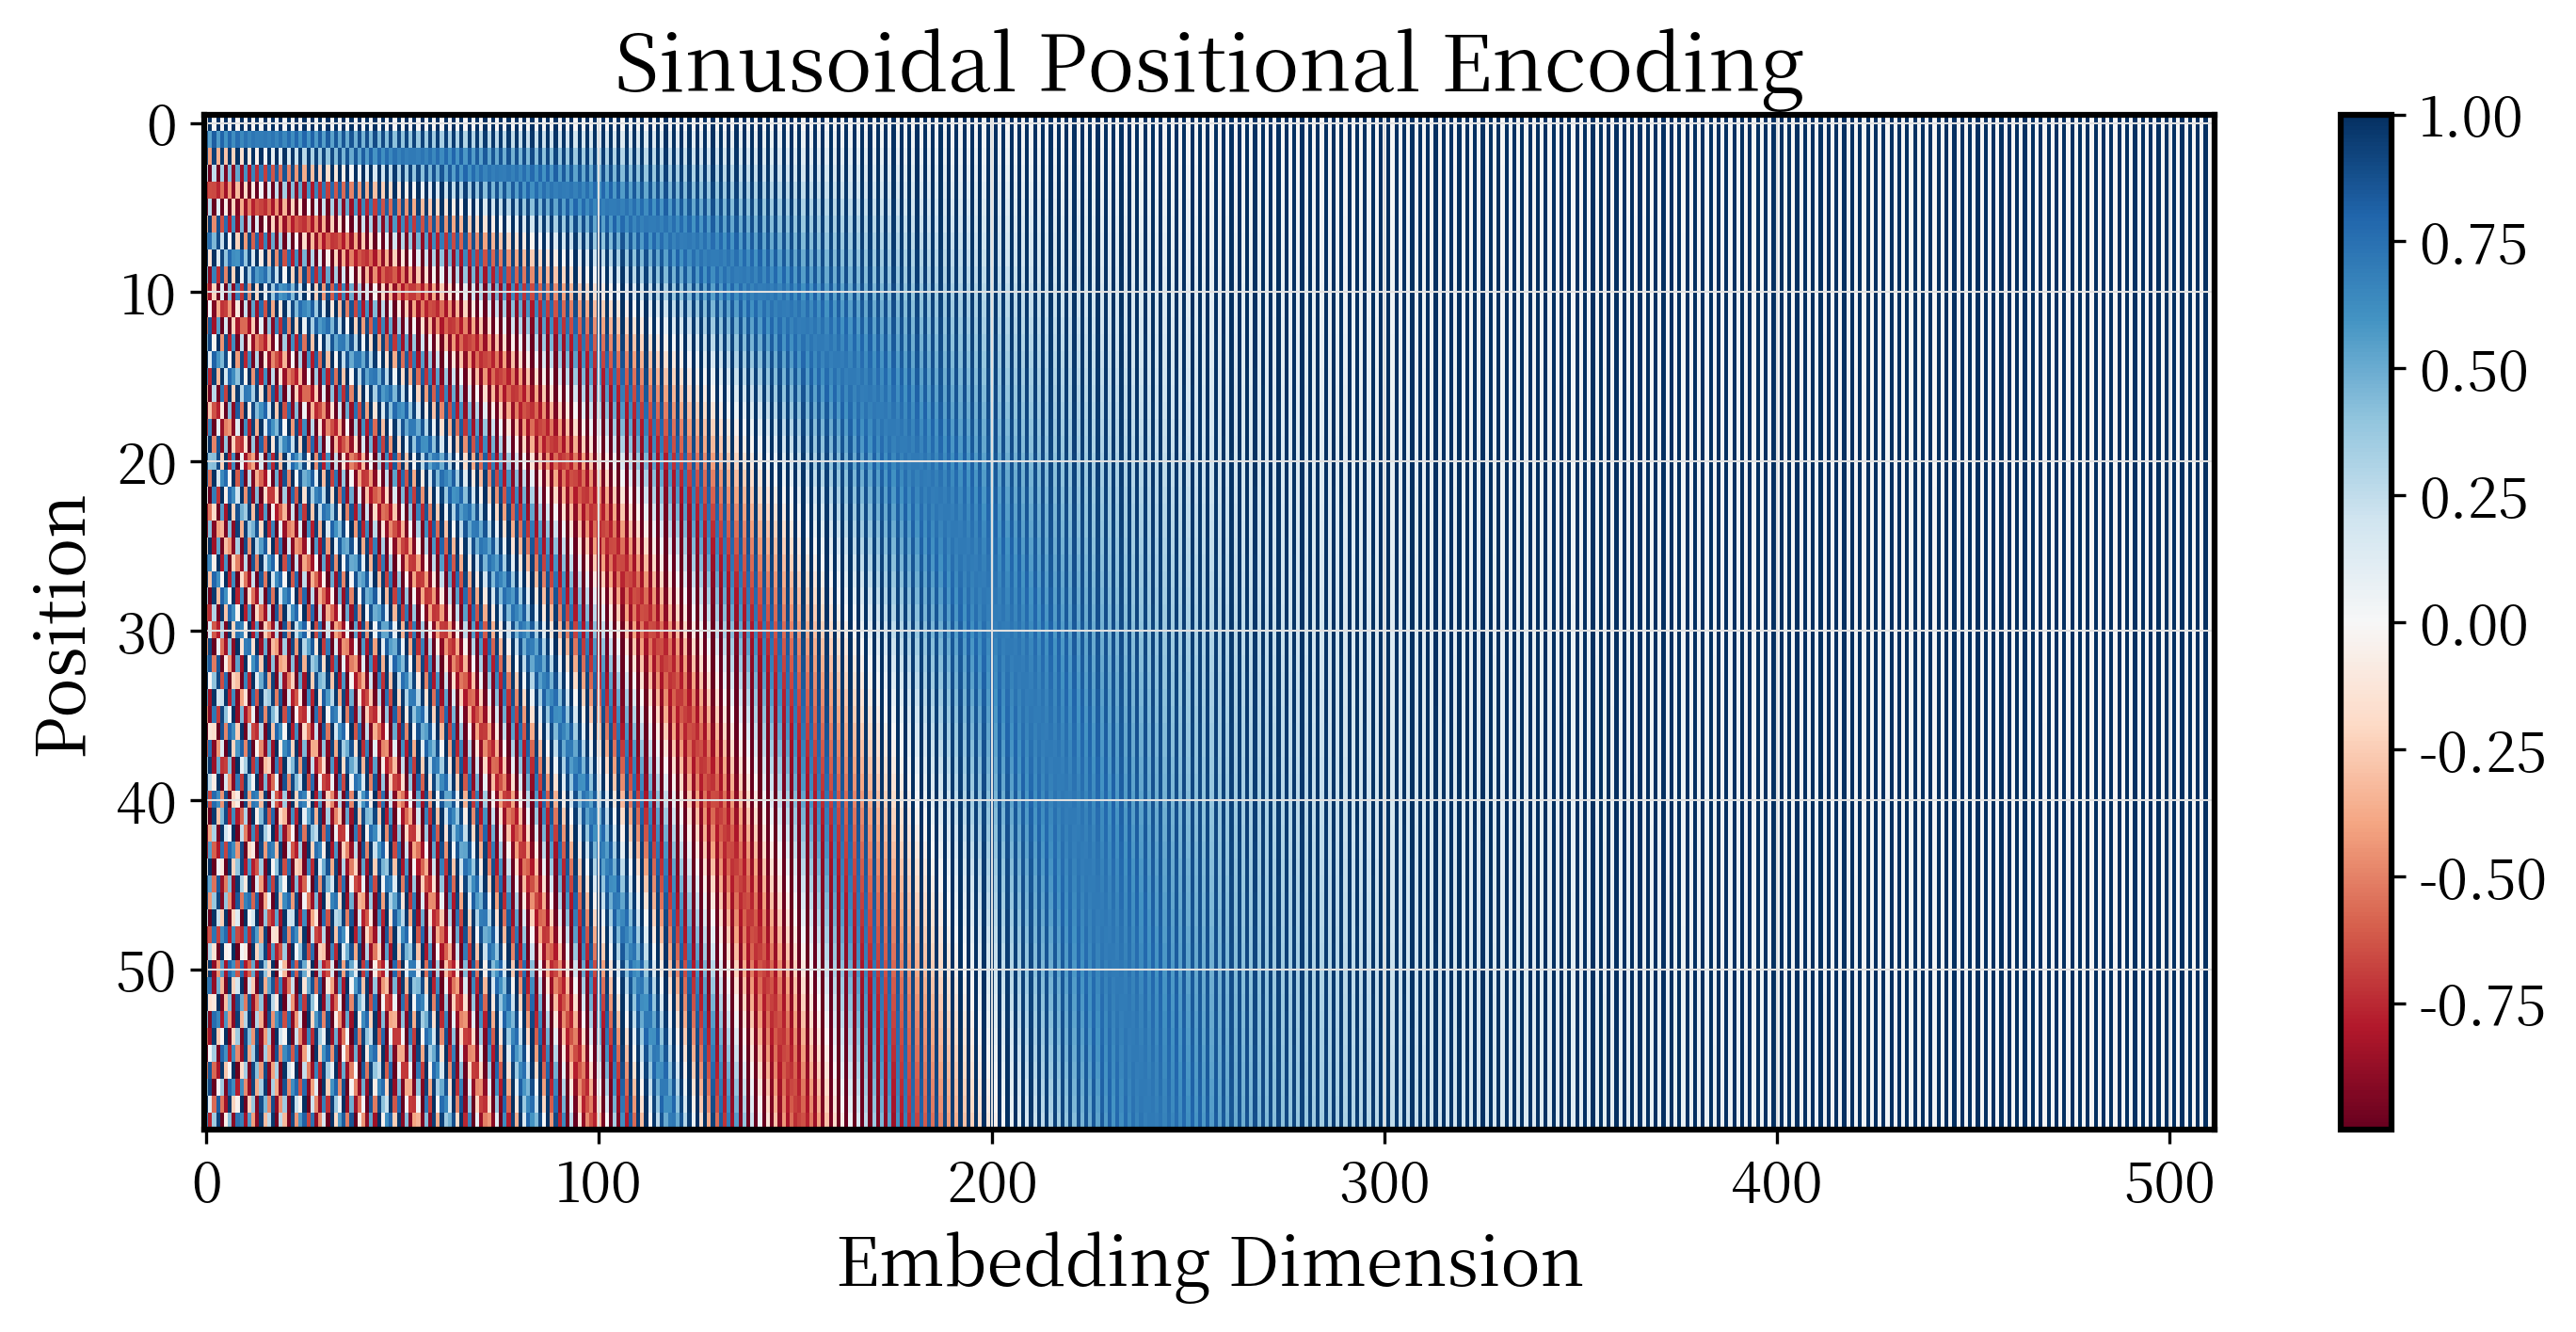
\includegraphics[width=0.8\textwidth]{figs/fig14_positional_encoding.png}
    \caption{正弦余弦位置编码可视化}
    \label{fig:pe}
\end{figure}

图\ref{fig:pe}展示了位置编码矩阵的结构。低维度的正弦波变化频率高，编码精细的位置信息；高维度的波形变化缓慢，捕捉全局位置关系。这种多尺度的编码方式使得模型能够同时感知局部词序和全局句子结构。

\subsection{训练效率}

\begin{figure}[H]
    \centering
    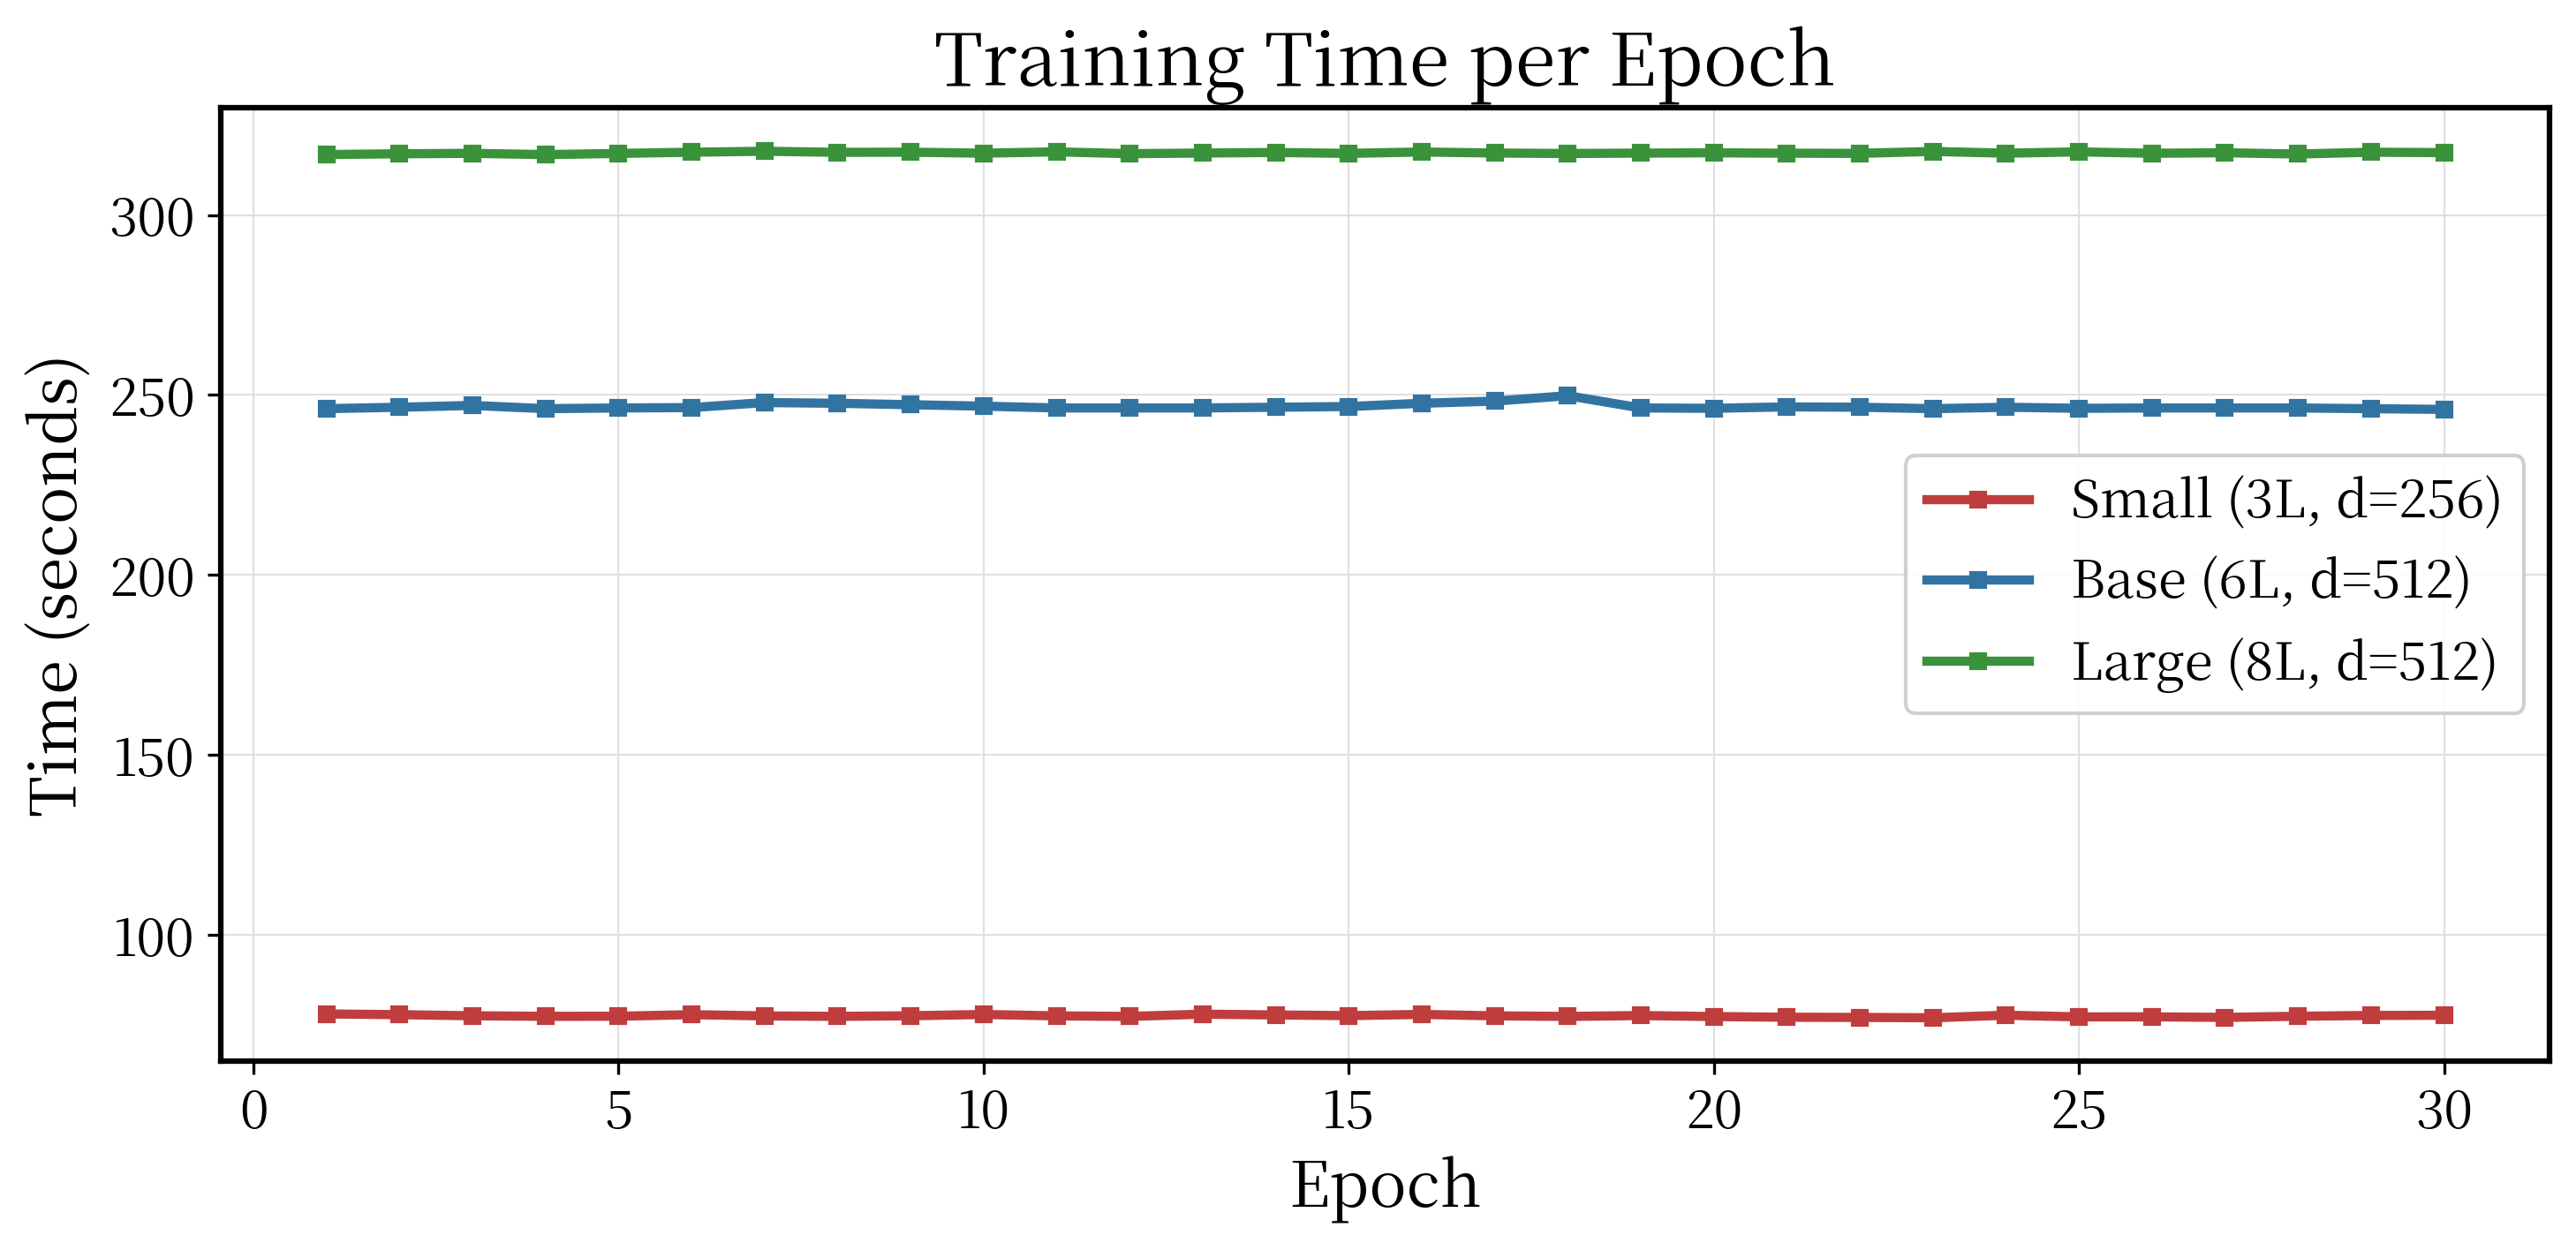
\includegraphics[width=0.95\textwidth]{figs/fig08_epoch_time.png}
    \caption{各模型每个epoch的训练时间}
    \label{fig:time}
\end{figure}

Transformer的一个显著优势在于并行化计算。自注意力机制可以同时计算所有位置之间的关系，GPU的并行能力得到充分利用。从图\ref{fig:time}可以看出，模型规模的增长并不会导致训练时间成比例增加，体现了Transformer在计算效率上的优势。

\subsection{翻译示例}

表\ref{tab:samples}展示了Base模型（beam=5）在测试集上的部分翻译结果，并与参考译文进行对比。

\begin{longtable}{p{0.08\textwidth}p{0.85\textwidth}}
    \caption{翻译示例对比（Base模型，beam=5）} \label{tab:samples} \\
    \toprule
    \endfirsthead
    \multicolumn{2}{l}{\small 续表\ref{tab:samples}} \\
    \toprule
    \endhead
    \bottomrule
    \endfoot
    \multicolumn{2}{l}{\textbf{示例1}} \\
    \midrule
    源文 & 在此 背景 下 , 中国 要 融入 世界 经济 , 有必要 加快 发展 高技术 产业 , 增强 综合 国力 , 改善 这 一 产业 的 国际 分工 地位 . \\
    译文 & against this backdrop , china must integrate its integration with the world economy , accelerate the development of high - tech industries , and enhance the overall national strength of the industry , thus improving the international division of labor . \\
    参考 & against this background , if china is to be incorporated into the world economy , it is essential that we accelerate the development of high - tech industry , enhance the overall national strength , and improve this industry 's standing in terms of the international division of labor . \\
    \midrule
    \multicolumn{2}{l}{\textbf{示例2}} \\
    \midrule
    源文 & 据介绍 , 全国 政协 港澳台 侨 委员会 去年 将对 台 工作 列为 工作 重点 . \\
    译文 & it has been learned that the work of the hong kong and macao affairs committee of the national committee of the cppcc and the taiwan affairs office was set up last year . \\
    参考 & as related , the hong kong , macao , taiwan , and overseas chinese committee under the national cppcc committee last year designated the work towards taiwan as the priority of its work . \\
    \midrule
    \multicolumn{2}{l}{\textbf{示例3}} \\
    \midrule
    源文 & 广大 发展中国家 也 意识到 , 只有 通过 参与 和 合作 , 才能 逐步 改变 不合理 和 不 公正 的 国际 经济 秩序 . \\
    译文 & the vast developing countries also understand that only through participation and cooperation can they gradually change their unfair distribution and the unfair distribution of international economic order . \\
    参考 & the developing countries have also realized that only through participation and cooperation can they gradually change the irrational and unfair international economic order . \\
\end{longtable}

从翻译示例中可以看出，模型已经学会了中英文之间的基本语序转换规则，能够正确处理常见的语法结构。对于示例1这类长句，模型成功捕捉到了"加快发展""增强""改善"的并列结构；但也存在语义偏差等问题，尤其在包含专有名词或复杂从句的长句中，翻译的准确性仍有提升空间。

\subsection{与RNN方法的对比}

相比实验3中基于LSTM/GRU的序列模型，Transformer在机器翻译任务上有明显优势：自注意力机制避免了信息在长序列中逐步衰减的问题，并行计算大幅缩短了训练时间，多头注意力能够在不同表示子空间中捕捉多样化的语言模式。不过Transformer参数量通常更大，在小规模数据集上需要注意过拟合风险。

\section{实验总结}

本实验完整实现了基于Transformer的中英机器翻译系统。通过对比三种不同规模的模型配置，发现在10万句对规模的训练集上，较小的模型（3层、256维）反而取得了最优的翻译质量，而过大的模型（8层、97.6M参数）由于欠拟合表现不佳。这一结果说明模型容量需要与数据规模合理匹配。实验中，配合Noam学习率调度、标签平滑和束搜索等技术，Base配置的Transformer模型在beam=5下达到了BLEU-4=14.80，满足实验要求。

本实验加深了我对注意力机制、位置编码和自回归解码等核心概念的理解，也让我认识到机器翻译系统的质量不仅取决于模型架构，还与数据质量、训练策略和解码方法密切相关。

本实验代码位于：\url{https://github.com/neverwinHao/deep-learning-project/tree/main/Exp4/code}

\end{document}
